\documentclass[b5paper, twoside, openright]{report}
% \documentclass[b6paper]{report}
% \usepackage[lmargin=25mm, rmargin=25mm, tmargin=27mm, bmargin=30mm]{geometry}
\usepackage[tmargin=27mm, bmargin=30mm]{geometry}

\usepackage[T1]{fontenc}
\usepackage[toc]{appendix}
\usepackage{amsmath}
\usepackage{amsthm}
\usepackage{amssymb}
\usepackage{color}
\usepackage{graphicx}
\usepackage[colorlinks, linkcolor=theme1, linktocpage,
            citecolor=theme2]{hyperref}
\usepackage{footnotebackref}
\usepackage[capitalize, nameinlink]{cleveref}
\crefname{lstlisting}{Listing}{Listings}
\usepackage[colorinlistoftodos,
            textsize=footnotesize,
            linecolor=none,
            bordercolor=none,
            backgroundcolor=none]{todonotes}
% \usepackage{libertinust1math}
\usepackage{euler}
\usepackage{libertine}
\usepackage{inconsolata}
\usepackage{listings}
% \usepackage{parskip}
\usepackage{wrapfig}
\usepackage{subcaption}
\usepackage{tikz}
\usetikzlibrary{positioning,shapes,decorations,decorations.markings,calc,fit,arrows.meta,backgrounds}
\usepackage[inline,shortlabels]{enumitem}
\usepackage{xcolor}
\usepackage{longtable}
\usepackage[automake,acronym]{glossaries}
\usepackage{titlesec}
\usepackage{blindtext}
\usepackage{microtype}
\usepackage{clrscode3e}

\usepackage{fancyhdr}
%   \fancyhf{}
\fancyhead[LO,RE]{\textsc{\leftmark}}
\fancyhead[RO,LE]{\textsc{\rightmark}}

\titleformat{\part}[display]
  {\center}
  {\Large\scshape{\partname} \thepart}
  {0ex}
  {\Huge}

\titleformat{\chapter}[display]
  {\center}
  {\large\scshape{\chaptertitlename} \thechapter}
  {0ex}
  {\huge}

\titleformat*{\section}{\Large}
\titleformat*{\subsection}{\large}
\titleformat*{\subsubsection}{\bfseries\normalsize}

\catcode`_=12
\begingroup\lccode`~=`_\lowercase{\endgroup\let~\sb}

% Hack to make parskip and amsthm go well together.
% \begingroup
%     \makeatletter
%     \@for\theoremstyle:=definition,remark,plain\do{%
%         \expandafter\g@addto@macro\csname th@\theoremstyle\endcsname{%
%             \addtolength\thm@preskip\parskip
%             }}
% \endgroup

\theoremstyle{plain}
\newtheorem{theorem}{Theorem}[chapter]
\newtheorem{lemma}[theorem]{Lemma}

\theoremstyle{definition}
\newtheorem{definition}[theorem]{Definition}
\newtheorem{example}[theorem]{Example}

\graphicspath{{./graphics/}}

\makeglossaries{}

\begin{document}

\renewcommand{\thepage}{\roman{page}}%

\begin{titlepage}
  \centering
  \null%
  \vspace{1cm}
  {\Large TDT4900: Masters Thesis \par}
  \vspace{2cm}
  {\huge CMR:\@ A concurrent memory\\ management system for Rust\par}
  \vspace{3cm}
  {\Large\itshape{}Martin Hafskjold Thoresen\par}
  \vfill
  supervised by\par
  {\large Magnus Lie Hetland}\\
  \vspace{2cm}
  {\large \today\\}
\end{titlepage}

\newcommand{\fixme}[1]{{\color{black}\todo{#1}}}

\newcommand{\code}[1]{{\color{darkred}\ttfamily #1}}
\newcommand{\mc}[1]{{\ttfamily #1}}
\newcommand{\coderef}[1]{(\texttt{#1})}

\newcommand{\rustc}{\code{rustc}}
\newcommand{\cargo}{\code{cargo}}
\newcommand{\rustup}{\code{rustup}}
\newcommand{\Operator}[1]{{\color{operator}#1}}

\tikzset{auto}
\tikzset{lnode/.style={node distance=2.5cm, rectangle split, rectangle
split horizontal, rectangle split parts=2, draw, rounded
corners=0.05cm,font=\footnotesize,fill=white}}
\tikzset{block/.style={regular polygon, regular polygon sides=4, draw, rounded
corners=0.02cm, font=\footnotesize}}
\tikzset{text/.style={regular polygon, regular polygon sides=4 }}
\tikzset{ptr/.style={{Circle[black, length=3pt]}-latex}}
\tikzset{ptr-g/.style={{Circle[lightgray, length=3pt]}-latex}}
% Dotted start for arrows.
\tikzset{
    circlebase/.style={
        decoration={
            markings,
            mark={
                at position 0
                with {
                    \draw [fill] circle [radius=#1];
                }
            }
        },
        postaction=decorate
    },
    circlebase/.default=0.5mm
}



\definecolor{lightblue}{HTML}{AFE0FF}
\definecolor{lightred}{HTML}{FFA0AF}
\definecolor{darkred}{HTML}{A02020}

\definecolor{rust}{HTML}{FFE7C7}
\definecolor{operator}{HTML}{004b84}

\definecolor{theme1}{rgb}{0.5,0.1,0.5}
\definecolor{theme2}{rgb}{0.1,0.5,0.5}
\definecolor{theme3}{rgb}{0.1,0.1,0.5}
\definecolor{none}{rgb}{1.0,1.0,1.0}


\newacronym{ipc}{IPC}{Inter-Process Communication}
\newacronym{tls}{TLS}{Thread-Local Storage}
\newacronym{pthreads}{{\code{pthreads}}}{POSIX threads}
\newacronym{nll}{NLL}{Non-Lexical Lifetimes}


\lstset{%
 backgroundcolor=\color{white},
 basicstyle=\footnotesize\ttfamily,
% breaklines=true,
% captionpos=b,
 commentstyle=\color{gray},
 columns=flexible,
 keywordstyle=\color{theme1},
%language=C,
 keywords={let,mut,fn,return,pub,struct,where,impl,as,match,not,if,else,loop,while,unsafe,default},
% morekeywords={*,
 numbers=none,
 numbersep=5pt,
 numberstyle=\color{gray}\ttfamily,
 showspaces=false,
 showstringspaces=false,
 frame=single,
 rulecolor=\color{lightgray},
 literate=
 {(}{{\Operator{(}}}1
 {)}{{\Operator{)}}}1
 {[}{{\Operator{[}}}1
 {]}{{\Operator{]}}}1
 {<}{{\Operator{<}}}1
 {>}{{\Operator{>}}}1
 {+}{{\Operator{+}}}1
 {-}{{\Operator{-}}}1
 {=}{{\Operator{=}}}1
 {;}{{\Operator{;}}}1
 {:}{{\Operator{:}}}1
 {.}{{\Operator{.}}}1
 {)}{{\Operator{)}}}1
 {|}{{\Operator{|}}}1
 {*}{{\Operator{*}}}1
 {!}{{\Operator{!}}}1
 {\&}{{\Operator{\&}}}1
 {\ }{{\Operator{\ }}}1
 {\{}{{\Operator{\{}}}1
 {\}}{{\Operator{\}}}}1
}


\par\break\null%
\vskip 0.1\vsize%
{\centering\section*{Abstract}}
\addcontentsline{toc}{chapter}{Abstract}

\blindtext{}

\vfill%
{\centering\section*{Sammendrag}}

\blindtext{}

\vfill\break%


\par\break\null%
\vskip 0.1\vsize%
{\centering\section*{Acknowledgements}}
\addcontentsline{toc}{chapter}{Acknowledgements}

\lorem{}

\vfill\break%



\tableofcontents%
\listoffigures%
% \listoftables%

\listoftodos[Resolve These Things]

\clearpage\null%
\clearpage\setcounter{page}{1}%breakbreak
\renewcommand{\thepage}{\arabic{page}}%
\part{Bing Bong}




\pagestyle{fancy}

\chapter{Introduction}

\clearpage

\section{idk}

This is a thesis blabla
\\
Something about memory management and parallel systems
\\
bing bong about CMR
\\
Motivation
\\
RQ\ ?


\chapter{Background}


\section{Garbage Collectors}

A \emph{Garbage Collector} usually refers to an automatic subsystem that handles memory management
without requiring programmer assistence. Many widespread language implementations,
including Java, Python, and Go, use a garbage collector, although the internal details of each
system varies greatly.

The job of the garbage collector is to identify memory segments that are no longer used by the
program. One way of doing this is to represent the program memory as a graph $G=(V, E)$ where $V$ is
all allocated memory segments and $(u, v) \in E$ if the region $u$ contains an address that is
inside the segment $v$. One consequence of this model is that memory addresses cannot be computed
from other values.


\section{Operating Systems}
\blindtext{}

\subsection{Virtual Memory}
\blindtext{}

\subsubsection{Memory Maps\label{sec:memory-map}}
\blindtext{}


\subsection{Threads and Processes}
\blindtext{}


\section{Programming Languages}
\blindtext{}


\section{Memory Reclamation}
\blindtext{}

\subsection{Hazard Pointers\label{sec:hazard-pointers}}
\blindtext{}

\subsection{Forkscan\label{sec:forkscan}}
\blindtext{}


\section{Related Works}
\blindtext{}

\subsection{Crossbeam}
\blindtext{}


\chapter{Rust\label{ch:rust}}


Rust is a new programming language focusing on safety, performance, and concurrency\cite{rust}.
The official first stable release, Rust 1.0, was released in May 2015, and a new version of the
language as well as the official compiler, \code{rustc}, is released every 6th week. The language
is developed as an open source project on the version control platform GitHub\cite{github} by over
2000 contributors as of May 2018\cite{rust-github}. The Rust project is organized into
\emph{teams}, such as the Core Team, the Compiler Team, and the Documentation Team. Many of the
members of the Rust teams are Mozilla employees, and Mozilla officially sponsors the Rust project.
The language has no formal specification, although all language changes are developed and
documented through an \gls{rfc} process. For a thorough introduction to Rust, see \cite{trpl}.


\section{Introduction}

Rust is a compiled language with a minimal runtime, similar to C and C++. \code{rustc} uses
LLVM\cite{llvm} as a compiler backend for code optimization and code generation. The performance of
Rust code is very similar to that of C and C++\cite{rust-perf}; variations are often due to the
lack of stable features like SIMD support, or from different compile time information given to LLVM
by either language.

Rust has many features from the ML family of programming languages, such as pattern matching and
tagged enums, and a rich type system with type inference. Most notably, and unlike most other
modern programming languages, Rust does not have a garbage collector. Despite this, Rust programs
does not handle memory management manually; memory management is typically done statically at
compile time by utilizing language features covered in the upcomming sections.

Rust uses \code{struct}s similar to C and C++ which can have \emph{methods}, but it does not have
inheritance. \code{Trait}s are similar to interfaces: they define methods and optionally an
implementation, and \code{struct}s \emph{implement} the \code{Trait}. Traits can even be
implemented for types that we have not defined ourselves, as long as we have defined the
\code{Trait}. This is useful, since it means we can extend types from the standard library, or from
other third party crates\footnote{A \emph{crate} is a project unit, similar to a library}.
Important \code{Trait}s include \code{Deref} (the \code{*} operator), \code{Clone} (values that are
clonable), and \code{Drop} (ran when a value is destroyed).

When an owned value leaves its scope, it is destroyed and its \code{Drop} method is ran. Primitive
types, such as \code{char} or \code{u32} does not have a \code{Drop} implementation, but types
which holds a resource, like allocated memory, often has. \code{String}  and \code{Vec<T>} are
common examples. \code{String} has a pointer to an internal buffer, which needs to be freed upon
destruction in order not to leak memory. This \code{free} call is done inside \code{String::Drop}.


\section{The Borrow Checker\label{sec:borrow-checker}}

A central concept in Rust is that of ownership. At any moment, an object has exactly one binding
which \emph{owns} the object. Ownership may be transfered (``\emph{moved}'', which is the default
behaviour), or it may be \emph{lended out}. Then the receiver is \emph{borrowing} the binding.
There are two types or borrows: immutable and mutable borrows.
One of the reasons to differentiate between mutable and immutable borrows, is references in Rust
can be either aliased, or mutable, but never both.  That is, if there is a mutable reference to
some object, then that reference has to be the \emph{only} reference. This ensures that immutable
references are never changed, which makes it simpler for the programmer to reason about the code
since we get referential transparency, in addition to that it enables more compiler optimizations.

Borrowed objects are in effect \emph{references} to some data, similiar to pointers or references
in other programming languages. While Rust does have raw pointers (see \cref{sec:unsafe-rust}), it
is rarely used, and passing values by reference is prefered.  The three types of ownership handling
is shown in \cref{fig:rust-ownership}. In \cref{fig:ownership-transfer} we move \code{x}, so
\code{x} is no longer usable after the last line, and an attempt to use it is caught as a compile
time error: \code{error[E0382]: use of moved value: `x`}. Since the caller of \code{foo} has
``sent'' the \code{Foo} to the function, it does no longer have to do any cleanup: this is now
\code{foo}s responsibility.

\cref{fig:immutable-borrow} shows immutable borrow of \code{x}; the function \code{foo} may use the
\code{Foo}, but it cannot mutate it. \cref{fig:mutable-borrow} shows a mutable borrow; now
\code{foo} may mutate the \code{Foo}. Note that the binding \code{x} also needs to be mutable in
order to borrow mutably.

\begin{figure}[ht]
  \begin{subfigure}{0.3\textwidth}
    \caption{Ownership transfer\label{fig:ownership-transfer}}
    \begin{lstlisting}
fn foo(f: Foo);
let x = ...
foo(x);\end{lstlisting}
  \end{subfigure}%
  \hfill
  \begin{subfigure}{0.3\textwidth}
    \caption{Immutable Borrow\label{fig:immutable-borrow}}
    \begin{lstlisting}
fn foo(f: &Foo);
let x = ...
foo(&x);\end{lstlisting}
  \end{subfigure}%
  \hfill
  \begin{subfigure}{0.3\textwidth}
    \caption{Mutable Borrow\label{fig:mutable-borrow}}
    \begin{lstlisting}
fn foo(f: &mut Foo);
let mut x = ...
foo(&mut x);\end{lstlisting}
  \end{subfigure}%
  \caption{The three types of ownership handling.\label{fig:rust-ownership}}
\end{figure}


Understanding the borrow checker is often a pain point for new programmers, and the period in which
new Rust programmers learns an intuition about how to structure programs within these rules is
often refered to as ``fighting with the borrow checker''.


\section{Lifetimes\label{sec:rust-lifetimes}}

Lifetimes is the second important concept in Rust. The idea of lifetimes is to reason about the
duration of the program execution in which some object is valid --- its lifetime. By tracking the
lifetime of all variables at compile time the Rust compiler is able to catch errors such as
returning function local variable addresses. \cref{lst:lifetimes} shows an example function
attempting to do this.  \begin{lstlisting}[style=Rust,label=lst:lifetimes]
fn foo(_a: &i32) -> &i32 {
  let num: i32 = 420;
  let r: &i32 = &num;
  r }
\end{lstlisting}
 Since Rust tracks the lifetime of all variables,
it knows that the lifetime of \code{num} is the same as that of the function body. The lifetime of
\code{r} is the same, as it is a reference to \code{num}. So when we try to return \code{r} in the
last line of the function, Rust realizes that the lifetime of the reference we return ends its life
at the end of the function; this is clearly not what we wanted, since it would make the returned
reference dead on arrival. Compilation fails with the following error: \code{error[E0597]: `num`
does not live long enough}.


Although Rust programmers may have to think about the lifetime of the variables, they seldom have
to write lifetime annotated functions, due to \emph{lifetime elison} --- the compiler can ususally
figure out the most general lifetime that fits the function. Functions may be annotated with
explicit lifetimes, for instance if it takes multiple references in which the relative difference
of the lifetimes of the references is important.
\code{struct}s can also be annotated with lifetimes, and in fact is required to be so if any of its
members are references. This is because the lifetime of the struct is bounded by the lifetime of
its member variables.
\begin{lstlisting}[style=Rust]
struct Person<'a> {
  age: i32,
  name: &'a str }
\end{lstlisting}
Should we have a function that crates a new \code{Person} we might want to annotate it explicitly,
if the function takes multiple references, but only one of these references is the \code{name}
field:
\begin{lstlisting}[style=Rust]
fn make<'x, 'y>(f: &'y File, n: &'x str) -> Person<'x> { ... }
\end{lstlisting}
This way we can convey the information that the resulting \code{Peron} should live as long as
\code{n}, but may outlive the file \code{f}.



\section{Unsafe Rust\label{sec:unsafe-rust}}

When talking about the Rust progrmaming language, one usually talks about a subset of Rust, called
\emph{Safe Rust}. In Safe Rust, there are no race conditions, mutable memory locations are never
aliased, and all pointer accesses are valid.  The real world, on the other hand, rarely offers
these guarantees, and the unfortunate truth which Rust programmers must deal with is that in order
to implement some of these safe abstractions we want (like \code{Vec}, \code{Mutex}, and
\code{Box}), some unsafety is required.  For this reason, Rust offers an escape hatch for some of
its rules: \emph{Unsafe Rust}.

The difference between Safe and Unsafe Rust is only four things. In Unsafe Rust one may:
\begin{enumerate*}[1) ]
    \item dereference raw pointers
    \item mutate statics
    \item call \code{unsafe} functions
    \item implement \code{unsafe} traits.
\end{enumerate*}
One way of thinking about the unsafety of ones codebase is that there should be no undefined
behaviour in safe code, no matter how the code looks like. In other words, it should be impossible
to mess up so badly as to invoke undefiend behaviour without typing \code{unsafe}.

Dereferencing raw pointers is naturally \code{unsafe}, as it is not possible to statically
guarantee that the address of the pointer is valid memory, or that the objects it points to is
still alive, nor that mutation of that memory does not change an immutable reference some other
place in the program. Mutation of \code{static} variables is also unsafe due to mutability of
aliased references, and due to the lack of thread synchronization.

\code{unsafe} functions and traits are just a marker added to the function or trait, signaling that
not all uses of this is guaranteed to be safe. As an example, the trait \code{Send} is a marker
trait and types implementing \code{Send} may be sent across thread boundaries. While this is fine
for most types, there are types which does not allow this. The reference counted pointer
\code{Rc<T>} is an example, which is a pointer to a tuple\footnote{Not really, but for our purposes
here we can pretend that it is.} \code{(count, data)}. The \code{count} is incremented each time
\code{.clone()} is called, and decremented when a variable is \code{Drop}ped.  To understand why
this cannot be send across thread boundaries safely, consider what happens if $T\sb{1}$
\code{.clone()} at the same time as $T\sb{2}$ \code{Drop}s it: the \code{count} field is written to
twice without any synchronizationor atomic operations\footnote{\code{Rc} does not use atomics for
performance reasons, but \code{Arc} does, and it does implement \code{Send}.} --- a race condition!



\section{Concurrency}

bing bong

\subsection{Concurrency and Aliasing\label{sec:concurrency-and-aliasing}}

One observation to make from the reference rules as presented in \cref{sec:borrow-checker} is that
since references are either aliased or mutable, then there can be no writes shared data between
threads, in Safe Rust, even using atomics. While this is \emph{technically} true, the Rust standard
library uses \code{\&T} and \code{\&mut T} slightly different than ``immutable'' vs ``mutable'' in
this context: \code{\&T} means that the type may be shared between threads.

Take \code{AtomicUsize} as an example, a \code{usize} exposing atomic operations like \code{store},
\code{load}, and \code{compare_and_swap}, which signatures are shown in \cref{lst:atomicusize}.
\begin{lstlisting}[label=lst:atomicusize,caption=Signatures for selected operations on
\code{AtomicUsize}]
fn load(&self, order: Ordering) -> usize;
fn store(&self, val: usize, order: Ordering);
fn swap(&self, val: usize, order: Ordering) -> usize;
fn compare_and_swap(&self, current: usize, new: usize, order: Ordering) -> usize;
\end{lstlisting}

Clearly, \code{AtomicUsize::store} modifies memory of the \code{usize}; despite this the function
is \code{\&self} and not \code{\&mut self}, since the operation is allowed on variables which are
shared between threads.
This is a useful distinction, since we can have methods on \code{AtomicUsize} that \emph{is}
\code{\&mut self}, which then is only possible to invoke should the variable not have been shared
between threads yet; we know this since this means that we have aliased mutable references, which
is not allowed. For instance, \code{AtomicUsize::get_mut(\&mut self) -> \&mut usize} allows the
underlying \code{usize} to be changed without any synchronization overhead.


\subsection{Common Patterns}

The standard librarys synchronization module \code{std::sync} contains primitives that most
concurrent programs require, such as \code{Mutex}, \code{Channels}, \code{Condvar}, and
\code{Atomic}s. A common pattern in Rust is the \gls{raii} pattern. The idea is that resources
should be managed automatically when constructing and destructing an object. \code{Mutex} uses
these ideas: \code{Mutex::lock} returns an \code{Result<MutexGuard>}, where the \code{MutexGuard}
wrapps a mutable reference to the data that is protected by the \code{Mutex}. When the
\code{MutexGuard} goes out of scope, its \code{Drop} implementation is ran, and the \code{Mutex} is
unlocked.

It is common among Rust programmers to build abstractions over lower level primitives. For
instance, a common pattern in parallel and concurrent programming is to have a \emph{thread pool},
which is given work, and internally handles the thread synchronization and work division. Example
usage of such an abstraction could be \code{let tp = ThreadPool::new(); tp.execute(|| { ... });}.
Since this can be implemented without any special compiler support, such crates are usually made as
third party libraries.

Another example is data parallelism: given some collection of data we want to iterate over the
elements and perform some operation on each element. The Rust library \code{rayon} offers exactly
this: parallel iterators. Instead of writing \code{vec.iter()} to iterate over a \code{Vec} and
then performing some operation on each element sequentially, with \code{rayon} we can write
\code{vec.par_iter()}, and get data parallelism for free. The operation is then ran in parallel
with any number of threads. Internally \code{rayon} uses a thread pool and work stealing to handle
the division of labour among the threads.


\fixme{09/05 12:32 Look at stuff from last semester. Move into std sec?}
\subsection{Memory Orderings}

\section{Nightly Rust}

The Rust language and compiler follows a fixed release schedule, where a new stable version is
released every six weeks. In addition to this there is the beta branch, which is the upcomming
version, and the nightly version which is the most recent version, build daily from the
\code{master} branch of the source tree.

The nightly version of the compiler allows users to opt in on \emph{untsable} features: features
that are partially or fully implemented, but which details are not yet committed to. These featuers
includes new APIs in the standard library, new syntax, and new language features all together.
As we have used multiple unstable features in CMR, we look at some of them in deatil.


\subsection{Non-Lexical Lifetimes\label{sec:nll}}
The current implementation of lifetime checking in the compiler is \emph{lexical}, meaning
variables are live until they go out of scope, despite not being used. This is a limitation that
one may want to get rid off. The feature \gls{nll} lifts this requirement, and lets the lifetime of
a variable last only until its last usage. Having this it is possible to seemingly break some of
Rust rules, like aliased mutable references:
\begin{lstlisting}[style=Rust]
let mut v = vec![1,2,3];
let r1 = &mut v;
let r2 = &mut v;
\end{lstlisting}

This clearly violates one of the Rust rules, namely that we cannot have mutable aliased referenes.
Yet, in this example we have two mutable references, \code{r1} and \code{r2}, to the same data.
With \gls{nll} this will compile, as we do not use \code{r1} after having made \code{r2}, so its
lifetime is implicitly ended right after its declaration. If we write \code{r1.push(1);} after
\code{let r2}, we get the same error as without using \gls{nll}, since the lifetime \code{r1}
overlaps with the lifetime of \code{r2}.



\subsection{Trait Objects\label{sec:trait-objects}}

When using traits in function signatures or structs we can either make the struct generic over some
type that implements the trait, or we can use dynamic dispatch. As generics usually are implemented
by copying the source code for the type for each invocation of a new type, it increases code size
and compilation time. In addition, collections and similar structures cannot mix different types: a
\code{Vec<SomeTrait>} cannot both contain elements of type \code{A} and \code{B}, even if both
implements \code{SomeTrait}.

Dynamic dispatch is the other option. Now variables are \emph{fat pointers}, containing both the
pointer to the data type, and a pointer to a \code{vtable}\footnote{the name \code{vtable} comes
from the C++ world, where function on abstract types are called \code{virtual} functions}, which
contains information about the function addresses for that type, as shown in
\cref{fig:trait-objects}. The entry in the \code{vtable} is all functions for some trait. With this
we can take any concrete type, and follow its vtable pointer, in order to find the implementation
of some trait function for that type. In \cref{fig:trait-objects}, both \code{Foo} and \code{Bar}
implements some trait which have a function named \code{fnc}. By following the pointers from the
stack, we get the data (left) and the function pointer (right). This way of implementing Trait
Objects are usually not mandated by any standard, but it is popular across different language
implementations nevertheless.

\begin{figure}[ht]
  \centering
  \begin{tikzpicture}[node distance=1cm]
\tikzset{lnode/.style={node distance=1.25cm, rectangle split, rectangle
         split horizontal, rectangle split parts=2, draw,font=\footnotesize}}

  \node [lnode]  (st1)                {bing \nodepart{second} bong};
  \node [lnode]  (st2) [below of=st1] {bing \nodepart{second} bong};
  \node [draw, inner sep=0mm, fit={(st1) (st2)}] {};
\end{tikzpicture}

  \caption{Illustration of memory when using Trait Objects.\label{fig:trait-objects}}
\end{figure}

While trait objects offers greater flexibility in the usage of traits, the pointer jumping leads to
worse cache behaviour which may have a large impact on performance, and important compiler
optimizations like inlining is impossible.



\subsection{Specialization\label{sec:specialization}}

Specialization is a feature which allows multiple implementations of a trait for the same type,
where the implementations are ordered by their specificity.

Assume we want to implement the trait \code{Debug} for a struct that is generic over some type
\code{T}: \code{Struct<T>}. We might want to have different implementations of \code{Debug}
depending on whether the generic parameter \code{T} implements \code{Debug} or not.
Specialization makes this possible.
\begin{lstlisting}[
  style=Rust,
  label=lst:specialization,
  caption=Using specialization to implement a trait twice.,]
impl<T> Trait for Struct<T> {
  default fn fmt(&self);
}
impl<T: Debug> Trait for Struct<T> {
  fn fmt(&self);
}
\end{lstlisting}


With only these two implementation it is clear which of the two we want for any type: if \code<T>
implements \code{Debug} we want the second, and if it does not, we want the first. However, if we
mix in yet another trait, \code{Clone}, such that we have a third implementation
\begin{lstlisting}[style=Rust]
impl<T: Clone> Trait for Struct<T> { ... }
\end{lstlisting}
it is no longer clear which implementation to use if \code{T} implements \emph{both} \code{Clone}
and \code{Debug}. The current implementation forbids such implemementations.


\subsection{Allocators\label{sec:allocators}}

The final nightly feature that we look at is \emph{allocators}. It is not yet possible to change
the default allocator in stable Rust, but a suggested API for creating new allocators and
specifying the default system wide allocator for Rust programs is avaiable by opting in on the
allocator feature. The feature defines a trait \code{GlobalAlloc} that defines functions analagous
to \code{malloc} and \code{free} from libc, and a attribute \code{\#[global_allocator]} to select
which allocator we want to use.

The default allocator for Rust is jemalloc\cite{jemalloc}. By using other external crates we can
use either the default system allocator, or jemalloc wrapped in our own allocator. This can be
useful if we want to do bookkeeping, gather statistics, or do any thread synchronization outside of
the actual allocator we are using.

\begin{figure}[ht]
\begin{lstlisting}[caption=Custom allocators wrapping jemalloc and the system allocator]
pub struct WrapJemalloc;
unsafe impl GlobalAlloc for WrapJemalloc {
    unsafe fn alloc(&self, layout: Layout) -> *mut Opaque {
        (*\lit{Do something before calling alloc}*)
        Jemalloc.alloc(layout) }
    unsafe fn dealloc(&self, ptr: *mut Opaque, layout: Layout) {
        (*\lit{Do something before calling free}*)
        Jemalloc.dealloc(ptr, layouer); } }

pub struct WrapSystem;
unsafe impl GlobalAlloc for WrapSystem {
    unsafe fn alloc(&self, layout: Layout) -> *mut Opaque {
        (*\lit{Do something before calling alloc}*)
        System.alloc(layout) }
    unsafe fn dealloc(&self, ptr: *mut Opaque, layout: Layout) {
        (*\lit{Do something before calling free}*)
        System.dealloc(ptr, layout); } }
\end{lstlisting}

\end{figure}


\chapter{CMR\label{ch:cmr}}

\fixme{09/05 13:22 remove impl stuff here. Should probably only talk about the system in an
abstract sense.}
We have named the system \emph{CMR}, short for \emph{Concurrent Memory Reclamation}. The system is
implemented as a Rust library \code{cmr}. We have also implemented four data structures, a stack,
queue, list, and hasmap, in the \code{cmr-data-structures} library, which uses \code{cmr}
internally for memory reclamation.

This chapter is organized as follows:
\cref{sec:cmr-overview} gives an overview of the system as a whole, and defines the problem
we want to solve.
\cref{sec:cmr-primitives} defines the primitives of the system, how they interact, and
proves their correctness.

\section{Problem Definition}

We define an abstract model of the system, and prove its correctness.
The computational model we are working with is the RAM\fixme{09/05 13:23 no} machine, and assume
that the reader is familiar with it.

We start by defining some central concepts.
Memory $M$ is the set of all addresses in the address space of the machine.
It is a disjoint set $M = A \cap F$ where $A$ is the set of allocated memory, and $F$ is the
remaining of the memory space.
A \emph{block} is a tuple $(addr, size)$ and represents the memory segment $\left[addr, addr +
size\right)$.
We call memory that is in an allocated block \emph{valid memory}.

In Rust, most memory management is handled automatically by the compiler. CMR utilizes this by
distinguishing between \emph{Rust memory} and \emph{Shared memory}. Rust memory is all memory that
is managed by the compiler, for instance through smart pointers. Shared memory is the remaining
memory, which is managed by CMR\@. Note that there is a thin line in between the two types: types may
be handled by CMR, but they themselves may contain smart pointers which is then handled by Rust.
For instance, a node in a linked list implemented using CMR may contain data that contains a smart
pointer. When the node is freed, its destructor is ran, and the smart pointers cleanup is handled
just as if it was not in shared memory (see \cref{fig:rust-shared-mem}).

Since Rust manages Rust memory, we only need to do reachability queries in the shared memory
subset. For many applications, this is a much smaller space than the total memory. It is also
possible to have the data types that are referenced from shared memory but stored in Rust memory
(like the binary tree in \cref{fig:rust-shared-mem}) know whether they have pointers to
shared memory, so that we don't have to scan through the strucutre, as it may be arbitrary large.


\begin{figure}
  \centering
  \begin{tikzpicture}
  \node [lnode,node distance=1.5cm] (n1)               {};
  \node [lnode,node distance=1.5cm] (n2) [right of=n1] {};
  \node [lnode,node distance=1.5cm] (n3) [right of=n2] {};
  \node [lnode,node distance=1.5cm] (n4) [right of=n3] {};

  \draw[ptr] ($(n1.east) - (0.25,0)$) -- (n2);
  \draw[ptr] ($(n2.east) - (0.25,0)$) -- (n3);
  \draw[ptr] ($(n3.east) - (0.25,0)$) -- (n4);
  \draw[ptr] ($(n4.east) - (0.25,0)$) -- ($(n4.east) + (0.4,0)$);

  \node [draw,fill=white,node distance=1.5cm, inner sep=0.2cm] (d1) [below of=n1,xshift=-0.19cm] {};
  \node [draw,fill=white,node distance=2cm,circle] (d2) [below of=n2,xshift=-0.19cm] {};
  \node [draw,fill=white,node distance=1.5cm] (d3) [below of=n3,xshift=-0.19cm] {$\pi$};
  \node [draw,fill=white,node distance=1.5cm] (d4) [below of=n4,xshift=-0.19cm] {\code{"hello"}};


  \draw[ptr] ($(n1) + (-0.19, +0.05)$) -- (d1.north);
  \draw[ptr] ($(n2) + (-0.19, +0.05)$) -- (d2.north);
  \draw[ptr] ($(n3) + (-0.19, +0.05)$) -- (d3.north);
  \draw[ptr] ($(n4) + (-0.19, +0.05)$) -- (d4.north);

  \node[draw,fill=white,circle,node distance=0.5cm] (treel) [below of=d2,left of=d2] {};
  \node[draw,fill=white,circle,node distance=0.5cm] (treer) [below of=d2,right of=d2] {};
  \draw[-latex] (d2) -- (treel);
  \draw[-latex] (d2) -- (treer);

  \node [draw,fill=white,node distance=2cm] (back) [left of=n1] {\code{0xcafe}};
  \draw[ptr] (back) ($(d1) + (0.05,0)$) to [out=180,in=270] (back.south);

  \begin{scope}[on background layer]
    \node [draw,fill=lightred!40, fit={(back) (n4)},inner sep=0.5cm] (shared-mem) {};
    \node [draw,fill=rust!60, fit={(d1) (treel) (d4)},inner sep=0.3cm] (shared-mem) {};
  \end{scope}

  \node (shared-label) [above of=back] {Shared memory};
  \node (rust-label) [below of=d4,xshift=-0.3cm] {Owned memory};
\end{tikzpicture}

  \caption{Example of memory layout showing Rust memory (beige) and shared memory (red). Types in
  shared memory may contain pointers to Rust memory, and vice versa.\label{fig:rust-shared-mem}}
\end{figure}

\subsection{Memory Hazards}

There are a number of possible hazards when managing memory manually. We first define three
hazards:

\begin{definition}[invalid-read\label{def:invalid-read}]
  Memory that has never been allocated is read.
\end{definition}

\begin{definition}[use-after-free\label{def:use-after-free}]
  Memory that was allocated and then freed is read.
\end{definition}

\begin{definition}[double-free\label{def:double-free}]
  A block is freed twice without being allocated in between.
\end{definition}

invalid-read is the least frequent of the three, as it requires the programmer to conjure a pointer
out of thin air, since it has never been allocated in the system.\ use-after-free is the most
hazarous of the three, as program behaviour is often undefined when freed values are read
\fixme{05/05 16:09 ref UB}; in many language implementations undefined behavious means that the
entire program is illegal, and one cannot assume anything about its behaviour.\ double-free is
technically not a memory hazard, as the operating system can check for the validity of pointers
that are freed. This is often not done in practice, and POSIXs definition of \code{free} states
that it is undefined behaviour to pass a non-allocated pointer to \code{free}\cite{posix}.

We will show that CMR guarantees that neither of the three hazards is possible in safe Rust.

\section{Overview\label{sec:cmr-overview}}

CMR is based on Forkscan\cite{alistarh2017forkscan}, but instead of scanning through the memory of
each thread, we take a different approach: The high level idea of the system is for the reclaiming
thread to have easy access to all roots in every thread. With this information, the problem of
identifying garbage is equivalent to reachability analysis in a graph in which the vertices are
data types in the program and the edges are pointers. Having this, we can identify the reachable
segments $R \subseteq M$ and the garbage $G = M \setminus R$.

\begin{figure}[ht]
  \centering
  \begin{subfigure}{0.45\textwidth}
    \begin{lstlisting}
a = Node { value = 4, next = null }
b = Node { value = 8, next = a }
list = [a, b, 3]
    \end{lstlisting}
  \end{subfigure}
  \hfill
  \begin{subfigure}{0.45\textwidth}
    \begin{tikzpicture}[node distance=1cm]
  \node [draw,circle,label={a}]    (a)              {};

  \node [draw,circle,label={b}]    (b) [right of=a] {};
  \draw[-latex] (b.west) -- (a.east);

  \node [draw,circle,label={3}]    (3) [right of=b] {};

  \node [draw,circle,fill,label={[label distance=-0.8cm]:list}] (l) [below of=a] {};
  \draw[-latex] (l.north) -- (a.south);
  \draw[-latex] (l.east) to [out=0,in=270] (b.south);
  \draw[-latex] (l.east) to [out=0,in=270] (3.south);


  \node [draw,circle,color=gray,label={[color=gray]x}] (x) [above of=b] {};
  \node [draw,circle,color=gray,label={[color=gray,label distance=-0.8cm]y}] (y) [right of=3] {};
  \draw[-latex,color=gray] (x.east) to [out=0,in=90] (y.north);
  \node [draw,circle,color=gray,label={[color=gray]z}] (z) [below of=3] {};
  \draw[-latex,color=gray] (z) -- (b);
\end{tikzpicture}

  \end{subfigure}
  \caption{Code sample (left) with possible heap layout (right). If the black filled node is the
  only root, the black nodes are reachable, and the gray nodes are not. Note that one node (z)
  points to a reachable node, but is itself not reachable.}
\end{figure}

Performing the reachability analisys is not straight forwards, even when we have all roots in the
system. Consider a mark-and-sweep approach, where we follow pointers and keep track of memory
locations that we have seen before. Since we are running a concurrent system, pointers might be
updated while we scan, so that two pointer values might be swapped after looking at either of them,
making the other value invisible to the system, and causing memory to be registered as unreachable,
when it is not. See \cref{fig:pointer-swap} for an example.

\begin{figure}[ht]
  \centering
  \hfill
\begin{tikzpicture}
  \node [draw,fill,circle] (r) {};
  \node [draw,circle] (a) [left  of=r, below of=r] {$a$};
  \draw[->,color=purple] (r) -- (a);
  \node [draw,circle] (b) [right of=r, below of=r] {$b$};
  \draw[->] (r) -- (b);
  \draw[<->,color=white] (a) to [out=-45,in=-135] (b);

  \node () [left of=r] {read left};
\end{tikzpicture}
\hfill
\begin{tikzpicture}
  \node [draw,fill,circle] (r) {};
  \node [draw,color=purple,circle] (a) [left  of=r, below of=r] {$a$};
  \draw[->,color=purple] (r) -- (a);
  \node [draw,circle] (b) [right of=r, below of=r] {$b$};
  \draw[->] (r) -- (b);
  \draw[<->,color=gray] (a) to [out=-45,in=-135] (b);
\end{tikzpicture}
\hfill
\begin{tikzpicture}
  \node [draw,fill,circle] (r) {};
  \node [draw,color=purple,circle] (a) [right  of=r, below of=r] {$a$};
  \draw[->,color=purple] (r) -- (a);
  \node [draw,circle] (b) [left of=r, below of=r] {$b$};
  \draw[->] (r) -- (b);
  \draw[<->,color=white] (b) to [out=-45,in=-135] (a);

  \node () [right of=r] {read right};
\end{tikzpicture}
\hfill

  \caption{Illustration of how mutation in the reachability graph can make a block $b$ appear as
  non-reachable. After we have looked at the left child of a node, but before reading its right,
  the nodes child pointers are swapped. Since we cannot detect that the pointers have been changed
  (the two pointers could have been the same), we see $a$ twice and do not see $b$.%
  \label{fig:pointer-swap}}
\end{figure}

In order to handle mutation problems, we obtain a snapshot of the entire processes memory by
freezing all threads, reading their roots, and forking the process. Thus, we have a snapshot of
the entire memory of the program, in which we also have all roots. Now the reachability analysis is
simpler, since there will be only one thread in the forked process, namely the garbage collecting
thread. \cref{lst:cmr} shows pseudocode for both the reclaiming thread and the other threads
for this procedure.

\begin{figure}[ht]
  \begin{subfigure}{0.45\textwidth}
    \begin{lstlisting}
CMR():
    freeze_threads()
    wait_for_writes()
    read_guards()
    fork()
    unfreeze()
    for addr in unreachables():
        free(addr)\end{lstlisting}
  \end{subfigure}
  \hfill
  \begin{subfigure}{0.45\textwidth}
    \begin{lstlisting}
on_freeze():
    write_roots()
    register_done()
    wait_for_unfreeze()\end{lstlisting}
  \end{subfigure}
  \caption{Pseudocode of CMR\@. The leftmost code is for the thread that runs the reclamation pass,
  and the rightmost code is other threads in the system.\label{lst:cmr}}
\end{figure}


\fixme{define ``Rust memory'' and shared memory}

\section{Primitives of CMR\label{sec:cmr-primitives}}

The central data type to achieve this is \code{Guard}. A \code{Guard} is an object in which a
pointer to shared memory is stored. All pointers to shared memory are stored in a Guard. By having
access to all \code{Guard}s, CMR have access to all roots in the program at any instant.
\code{Guard}s are similar to \gls{hps} (\cref{sec:hazard-pointers}), except that no thread
synchronization is performed when making new or updating existing \code{Guard}s, which reduces the
overhead of CMR significantly compared to \gls{hps}.

CMR has four types that are essential to understanding how we manage safe access to shared memory:
\emph{Guard}, \emph{Atomic}, \emph{NullablePtr}, and \emph{Ptr}. All types are generic over the
type of the data they protect, which is omitted for brevity.


\begin{definition}[Guard\label{def:guard}]
  A \emph{Guard} is an object that contains a \emph{root} or $\bot$. The Guard is non-movable in
  memory. All roots are stored in Guards.
\end{definition}

\begin{definition}[Atomic]
  An \emph{Atomic} is a pointer type that provides safe concurrent access to its users.
\end{definition}

\begin{definition}[NullablePtr]
  \emph{NullablePtr} is an immutable pointer that may be $\bot$. It is obtained through a Guard.
  When a NullablePtr $p$ is obtained from a Guard $g$, $g$ is immutable thoughout the
  lifetime\footnote{We use the same meaning of lifetime as Rust (\cref{sec:rust-lifetimes})}
  of $p$.
\end{definition}

\begin{definition}[Ptr]
  \emph{Ptr} is an immutable pointer that may \emph{not} be $\bot$. Its semantics are similar to
  that of NullablePtr, but the two are distinct types for simplification of the null-case. All
  accesses to shared memory is through a Ptr.
\end{definition}

These four types are the building blocks of writing concurrent structures in CMR\@. All pointers
are stored in an \mc{Atomic}, and loading an atomic using a \mc{Guard} yields a \mc{NullablePtr},
which may be promoted to a \mc{Ptr}, if it is not null. The \mc{Ptr} provides access to the data
the pointer points to.  In addition to having the types, CMR defines a number of operations that
acts on these types.  We look at each type in turn, and define their operations.

\subsection{Guard}
A Guard can be constructed with the initial value of $\bot$ with \emph{make-guard}
\begin{equation}\label{eq:make-guard}
  \text{make-guard\:::\:} () \to Guard
\end{equation}
It can also copy the value of another Guard with \emph{copy-guard}.
\begin{equation}\label{eq:copy-guard}
  \text{copy-guard\:::\:} (Guard, Guard) \to ()
\end{equation}

General usage of \mc{Guard} is to construct the number of \mc{Guard}s one needs for some operation.
These \mc{Guard}s are then used to load \mc{Atomic}s into.


\subsection{Atomic}

Atomic is a regular atomic pointer variable, supporing operations such as \emph{store}, and
\emph{compare-and-swap}.
\begin{equation}\label{eq:atomic-store}
  \text{store\:::\:} (Atomic, NullablePtr) \to ()
\end{equation}
\begin{equation}\label{eq:atomic-cas}
  \text{compare-and-swap\:::\:} (Atomic, NullablePtr, NullablePtr) \to NullablePtr
\end{equation}

It is not safe to \emph{load} an atomic, as there is no guarantee that the
pointer read is protected by a guard. Instead, CMR defines \emph{load-atomic}, which loads an
Atomic into a Guard, and returns the value read as a NullablePtr:
\begin{equation}\label{eq:load-atomic}
  \text{load-atomic\:::\:} (Guard, Atomic) \to NullablePtr
\end{equation}

\subsection{NullablePtr}

The NullablePtr is just a convenience type in order to not have to handle the $\bot$ case of all
pointers. Whether the pointer is null or not can be checked:

\begin{equation}\label{eq:nullable-is-null}
  \text{is-null\:::\:} (NullablePtr) \to bool
\end{equation}

CMR also supports using the lower bits of a pointer to store extra information (a \emph{tag}). This
is useful for implementing deletion in linked lists, among other things.  The tag is read with
\emph{tag},
\begin{equation}\label{eq:ptr-tag}
  \text{tag\:::\:} (NullablePtr) \to int
\end{equation}
and a new NullablePtr can be constructed with a given tag using \emph{with-tag}.
\begin{equation}\label{eq:ptr-with-tag}
  \text{with-tag\:::\:} (NullablePtr, int) \to NullablePtr
\end{equation}
The actual address is obtained through \emph{addr}
\begin{equation}\label{eq:ptr-addr}
  \text{addr\:::\:} (NullablePtr) \to int
\end{equation}

\subsection{Ptr}

\fixme{Reconsider having NullablePtr in here. I think its mostly a rust impl thing, as we just want
Deref on Ptr but must handle null as well.}
Ptr may be used in the place of NullablePtr, since is it just a special case of it. All functions
that take a NullablePtr can also take a Ptr.


\subsection{Other actions}

We also need a few other operations to make sure that the implementation of funcions are valid.
For instance, in load-atomic there is a window in between reading the atomic and storing the
pointer read it in the guard in which a reclamation pass may have happened. The higher order
function \emph{without_reclamation} makes sure that this is safe, by running the given function
without a reclamation pass happening in between:
\begin{equation}\label{eq:without_reclamation}
  \text{without_reclamation\:::\:} (() \to T) \to T
\end{equation}

As CMR controls memory allocations, it also defines its own allocation function:
\begin{equation}\label{eq:alloc}
  \text{alloc\:::\:} (Guard, T) \to Ptr
\end{equation}


\section{Correctness}

With these types and operations we are able to prove important properties of the system.

\begin{theorem}[\mc{Guard} is valid]\label{thm:guard-valid}
  If a \mc{Guard} is not $\bot$, it points to valid memory.
\end{theorem}
\begin{proof}
  Since the \mc{Guard} $g \neq \bot$, it has loaded its value from an Atomic $a$ using
  \mc{atomic-load}.  We first show that $a$ is itself in valid memory by induction: \emph{Base
  case:} the Atomic resides in Rust memory, and is thus valid. \emph{Inductive case:} the
  \mc{Atomic} resides in shared memory, and thus accessed through a \mc{Ptr} $p$.  This \mc{Ptr} is
  protected by a \mc{Guard} $g\sb{2} \neq g$, since $g\sb{2}$ is immutable throughout the lifetime
  of $p$, and $g$ is being changed. $g\sb{2}$ is valid by induction, so the pointer value in $a$ is
  reachable. This shows that the value read from the \mc{Atomic} is valid.

  Using \mc{without_reclamation} (\cref{eq:without_reclamation}), we make sure that the read of $a$
  and the store in $g$ happens without a reclamation pass in between. Thus all valid pointers
  before the read is still valid after the store. After the store operation in $g$ has completed,
  $g$ protects $v$. Thus $v$ is valid.
\end{proof}

\begin{lemma}[\mc{Ptr} is valid]\label{lm:ptr-valid}
  The \mc{Ptr} points to valid memory.
\end{lemma}
\begin{proof}
  The  \mc{Ptr} $p$ is read from a \mc{Guard} $g$ and $g$ is immutable throughout the lifetime of
  $p$ so they have the same value. $p \neq \bot$, so this follows by \cref{thm:guard-valid}.
\end{proof}

\cref{lm:ptr-valid} is the most important result in this section, since it guarantees that
accesses of the memory in a \mc{Ptr} is valid. Thus, a memory access through a \mc{Ptr} can not
result in a invalid-read (\cref{def:invalid-read}) or use-after-free (\cref{def:use-after-free})
hazard.



\part{Abcdef}

\chapter{Implementation\label{ch:implementation}}

\epigraph{Talk is cheap. Show me the code.}{\textit{Linus Torvalds}}

In this chapter we look at the Rust implementation of CMR\@. The source code is openly available
on GitHub under the MIT license~\cite{cmr-github}.

This chapter is organized as follows: \cref{sec:impl-data} discusses briefly the most important
data that CMR defines, both global and thread local;
\cref{sec:impl-primitives} shows the implementation of the primitives from
\cref{sec:cmr-primitives}, and argues for their correctness by the definitions in the previous
chapter;
\cref{sec:impl-snapshot} explains how memory snapshotting, an important part of CMR, is
implemented;
\cref{sec:impl-reachability} describes the reachability analysis including important details of the
Rust type system;
\cref{sec:impl-communication} mentions how communication between the parent and child process;
we finish the chapter with \cref{sec:impl-complications} where we highlight a few of the
complications that we encountered during the implementation of CMR.

\clearpage

\section{Data\label{sec:impl-data}}

In order to better understand how CMR is laid out, we start out by looking at the data.
As Fred Brooks~\cite{brooks1995mythical} said:
\begin{displayquote}
Show me your flowcharts and conceal your tables, and I shall continue to be mystified. Show me your
  tables, and I won't usually need your flowcharts; they'll be obvious.
\end{displayquote}

Allocated addresses are stored in a global \code{HashSet}, \code{ALLOCS}, which uses a \code{Mutex}
for thread synchronization. Only addresses in \code{ALLOCS} are subject for reclamation.
\cref{sec:impl-trace} explains more about the way allocations are stored in order to preserve type
information.

Thread also stores data in \gls{tls}. Each thread maintains a \code{Vec} of pointers to their
\code{Guard}s, such that collecting all guards is just a matter of iterating through the
\code{Vec}, and following the pointer. Since the data is thread local, no synchronization is needed
when operating on the \code{Vec}, which makes updates cheap.
In addition all threads store the allocations they have done since the last reclamation pass;
these allocations are ``stolen'' by the reclaiming thread in each pass. See
\cref{sec:impl-signalvec} for the details.

One caveat of CMR is that new threads needs to register themselves before using the system. This is
done through \code{cmr::register_thread()}. This initializes thread local data, and pushes a thread
handle used in \cref{sec:impl-snapshot}. We summarize some of the problems in
\cref{sec:impl-thread-registration}, and note that this is still a pain point of the
implementation.

Only one thread may be in a reclamation pass at any given time, and we limit this by having a
global \code{reclaim_lock}. A thread wanting to reclaim grabs the lock before doing anything else
in the reclamation procedure; this lock is later freed (see
\cref{sec:impl-communication}). If a thread attempts to do a reclamation pass but finds that the
lock is taken, it simply does not do the pass; waiting for the lock to be released would only
increase the latency of the reclamation pass for that thread, and since a reclamation pass was
recently performed, chances are that there will be very few new allocations to free in the pass.



\section{Primitives\label{sec:impl-primitives}}

In this section we present implementation of the primitives as presented in
\cref{sec:cmr-primitives}, and show that the implementation is unifiable with the definitions of
\cref{ch:cmr}. All \code{struct}s are shown with their full definitions, but we show only
highlights of the methods of the \code{struct}s, as most of them are trivial.

\subsubsection{Guard}

The \code{Guard} is implemented as a single word, in addition to an empty type (the
\code{PhantomData}) as Rust requires generic types to be used. \code{Guard}s aren't normally
constructed directly, but rather declared with the \code{guard!} macro, which constructs it and
calls \code{Guard::register}.  An excerpt of the definitions of \code{Guard} is shown in
\cref{lst:guard-impl}.

\begin{figure}
\begin{lstlisting}[style=Rust,
caption=Excerpt of \mc{Guard}s definitions,label=lst:guard-impl]
struct Guard<T> {
  ptr: usize,
  _marker: PhantomData<T>,
}
impl<T: Trace> Guard<T> {
    pub unsafe fn new() -> Self { Guard { inner: 0, _marker: PhantomData, } }
    pub fn copy_guard(&mut self, other: &Self) { self.inner = other.inner; }
    pub fn register(&mut self) {
        ROOTS.with(|r| { let mut v = r.borrow_mut();
                         v.push(GuardPointer::from_guard(self)) });
    }
    ...
}
macro_rules! guard {
    ($var:ident) => { let $var = unsafe { &mut $crate::guard::Guard::new() };
                      $var.register();
    }
}\end{lstlisting}

\end{figure}

\code{Guard::register} gets a mutable reference to the thread local \code{Vec} of \code{Guard}s,
and inserts a pointer to itself into it. \code{Guard::drop} (omitted) does the opposite.
\code{Guard::new} is marked \code{unsafe} since the caller must guarantee to \code{register} the
guard before using it. This is normally handled by the \code{guard!} macro, but there are use cases
for calling \code{new} directly. Usage of the guard is normally as follows:
\begin{lstlisting}[style=Rust]
{
  guard!(g);
  let my_num = cmr::alloc(123, g);
  println!("{}", my_num); // prints `123`
} // `g` is dropped here, and `my_num` is ripe for deallocation
\end{lstlisting}
Note that by using \code{guard!}, the caller only obtains a \code{\&mut Guard<T>}, and not the
\code{Guard<T>} itself; this makes it impossible to move the \code{Guard} in memory.


\subsubsection{Atomic}

\code{Atomic} is mainly a wrapper around Rusts \code{AtomicPtr}, although the internals differ
slightly. CMR defines its own type so that we can control the return types of certain functions.
\cref{lst:def-atomic} shows the definition of the \code{struct}, as well as \code{cas}, the
compare-and-swap operation, in which we utilize some Traits from the Rust standard library to
convert between types.  Implementation of remaining methods are straight forward.

\begin{lstlisting}[caption=Excerpt of \mc{Atomic}s definitions (Trait bounds omitted for brevity)]
pub struct Atomic<T> {
    data: AtomicUsize,
    _marker: PhantomData<T>,
}
impl<T> Atomic<T> {
    pub fn cas<'a, A, B>(&self, a: A, b: B, ordering: Ordering)
     -> Result<A, NullablePtr<'a, T>> {
        let (old, new£ = (raw(a£, raw(b££;
        let ret = self.data.compare_and_swap(old, new, ordering£;
        if ret == old { Ok(A::try_from(NullablePtr::new(ret££.unwrap(££ }
        else { Err(NullablePtr::new(ret££ }
    }
    ...
}

\end{lstlisting}


\pagebreak
\subsubsection{NullablePtr}

\code{NullablePtr} is used as the canonical pointer type in CMR, and all pointer like types are
converted to \code{NullablePtr} using the \code{From} and \code{Into} traits from the Rust standard
library, which handles conversion between types. For instance, we implement \code{From<*const T> for
NullablePtr<T>}. This way we can write functions that are generic over all types of pointers, so
that the user of CMR does not have to handle these conversions themselves.


The definition of \code{NullablePtr} is shown in \cref{lst:def-nullableptr}, with the \code{new}
and \code{ptr} methods. Note that we cannot get a reference to the \code{T} that \code{NullablePtr}
points to; this is because we don't know if the pointer is \code{null} or not. \code{ptr} promotes
the \code{NullablePtr} to a \code{Ptr}, should it not be \code{null}, by using the \code{Option}
type which Rust provides.

\begin{figure}[ht]
  \begin{lstlisting}[style=Rust,label=lst:def-nullableptr,
  caption=Definition of \code{NullablePtr}]
pub struct NullablePtr<'a, T: 'a>(usize, PhantomData<&'a T>);
impl<'a, T> NullablePtr<'a, T> {
    pub fn new(u: usize) -> Self { NullablePtr(u, PhantomData) }
    pub fn ptr(self) -> Option<Ptr<'a, T>> {
        if addr(self) == 0 { None }
        else { unsafe { Some(Ptr::new(raw(self))) } }
    (*\lit{\dots Remaining methods}*) }
\end{lstlisting}
\end{figure}


\subsubsection{Ptr}

\code{Ptr} provides access to the type it points to, as it is guaranteed to be non-\code{null}.
This is done through the \code{Deref} trait, which handles the \code{*} operator in Rust. Due to
auto-deref, we can now use \code{\&Ptr<T>} in place of a \code{\&T}. The definition of \code{Ptr},
a new of its methods, and its \code{Deref} implementation is shown in \cref{lst:def-ptr}. Node that
both \code{new} and \code{get_mut} are \code{unsafe} methods; \code{new} because we can not
guarantee that the address passed is valid, and \code{get_mut} because the data may be aliased.

\begin{figure}[ht]
  \begin{lstlisting}[style=Rust,label=lst:def-ptr,
  caption=Definition of \code{Ptr},
  escapeinside={(@}{@)},
  ]
pub struct Ptr<'a, T: 'a> { data: usize, _marker: PhantomData<&'a T> }
impl<'a, T> Ptr<'a, T> {
    pub(crate) unsafe fn new(u: usize) -> Self {
        Self { data: u, _marker: PhantomData, } }
    pub unsafe fn get_mut(&mut self) -> &mut T { &mut *self.as_raw() }
    fn as_raw(&self) -> *mut T { with_tag(*self, 0).data as *mut T }
    (@\lit{\dots Remaining methods}@) }
impl<'a, T> Deref for Ptr<'a, T> {
    type Target = T;
    fn deref(&self) -> &T { unsafe { &*(self.as_raw()) } } }
\end{lstlisting}
\end{figure}


\subsubsection{Tagging}

By having one canonical pointer type, we can define functions that are generic over all types
that supports conversion from and/or to \code{NullablePtr}. This is used in the functions for
pointer tagging, as well as the \code{cas} in \cref{lst:def-atomic} (the types \code{A} and
\code{B}). \cref{lst:tagging} shows some of the free functions for pointer tags that are generic
over different pointer types.

\begin{figure}[ht]
\begin{lstlisting}[
  numbers=left, numberstyle=\color{gray}\ttfamily{}TA,
  caption=Implementation of pointer tagging functions,
  label=lst:tagging]
pub fn tag<'a, P, T: 'a>(p: P) -> usize where P: Into<NullablePtr<'a, T>> {
    let n: NullablePtr<T> = p.into();
    n.0 & ones(TAG_BITS) }

pub fn with_tag<'a, P, T: 'a>(p: P, tag: usize) -> P
where P: Into<NullablePtr<'a, T>> + TryFrom<NullablePtr<'a, T>> {
    let p = p.into();
    let n = (p.0 & !(ones(TAG_BITS))) | tag;
    P::try_from(NullablePtr::new(n)).unwrap_or_else(|_e| panic!("failed conversion")) }


\end{lstlisting}

\end{figure}

\code{ones(k)} returns the bit mask with the \code{k} lower bits set, and \code{TAG_BITS} is a
predefined number of bits allowed to use for tagging for any pointer. We convert from \code{P} to
\code{NullablePtr} with \code{.into()} \coderef{TA2}.  In \code{with_tag} \coderef{TA5} we need
to use \code{TryFrom}, which is a conversion trait that may fail. In CMR \code{Ptr<T>} implements
\code{TryFrom<NullablePtr>}, where the conversion fails if the \code{NullablePtr} is \code{null}. We
assert that this failure should never happen \coderef{TA9} with the rationale that if we converted
some type \code{P} into a \code{NullablePtr} and changed its tag, we should be able to convert back
to \code{P}, even though the conversion is not always possible in general.

\subsection{Free Functions}

Having looked at the types and their member functions we now look at the implementations of
important free functions.

We first look at the higher order function \code{without_reclamation}:
\begin{lstlisting}[style=Rust]
pub fn without_reclamation<R, F: FnOnce() -> R>(f: F) -> R {
    let lock = ALLOC_LOCK.lock();
    compiler_fence(SeqCst);
    let ret = f();
    compiler_fence(SeqCst);
    drop(lock);
    ret }
\end{lstlisting}
The function runs the given closure without having a reclamation pass happening in between.  The
function simply grabs the reclamation lock before executing; is it however important that the
overhead here is as low as possible, as this is used in other important functions. For this reason
CMR also has the \code{without_reclamation_repeat} function, with attempts to run the closure
without any synchronization; if a reclamation pass happened while running, we rerun the function.

With the ability to run arbitrary code without a reclamation pass happening in between we can
implement \code{guard}, which is \proc{Load-Atomic} (\cref{eq:load-atomic}).
\begin{lstlisting}[style=Rust]
pub fn guard<'a, T>(guard: &'a mut Guard<T>, a: &Atomic<T>) -> NullablePtr<'a, T> {
    without_reclamation_repeat(|| { let p = unsafe { a.load(SeqCst) };
                                    guard.inner = ptr::raw(p);
                                    p }) }
\end{lstlisting}
Since we guarantee that no pass happened in between reading the \code{Atomic} and protecting the
data it pointed to in the \code{Guard}, we know that the data is still valid.


Another important function is \code{alloc}, which allocates memory:
\begin{lstlisting}[style=Rust]
pub fn alloc<T: Trace>(guard: &mut Guard<T>, t: T) -> Ptr<T> {
    let ptr = alloc::alloc(t);
    guard.inner = ptr::addr(ptr);
    alloc::register(ptr);
    ptr }
\end{lstlisting}
Note that we do not need to use \code{without_reclamation} here, since the newly address is
protected by the \code{Guard} before being registered; recall from \cref{sec:impl-data} that only
registered allocations are subject for reclamation.




\subsection{Correctness}

We argue for the correctness of the primitives as presented with respect to the definitions from
\cref{ch:cmr}.


\begin{claim}
  \cref{def:load-atomic-no-reclamation} is achievable.
\end{claim}
\begin{proof}
  \code{guard} implements \proc{Load-Atomic} with the wanted semantics.
\end{proof}

\begin{claim}
  \code{Guard} satisfies \cref{def:guard}.
\end{claim}
\begin{proof}
  The \code{Guard} is constructed with \code{null}, and gets values from \code{Atomic}s using
  \code{cmr::guard}; the values read are roots.
  Using the \code{guard!} macro it is impossible to move the \code{Guard}.
\end{proof}

\begin{claim}
  \code{NullablePtr} satisfies \cref{def:nullable-ptr}.
\end{claim}
\begin{proof}
  The type does not expose any mutating methods, so it is immutable.
  Looking at the function \code{guard} we see that the \code{\&mut Guard} is mutably borrowed, and
  since the lifetime of the \code{NullablePtr} returned has the same lifetime, the \code{Guard} is
  borrowed for the lifetime of the \code{NullablePtr}
\end{proof}

\begin{claim}
  \code{Ptr} satisfies \cref{def:ptr}.
\end{claim}
\begin{proof}
  The type does not expose any mutating methods, so it is immutable.
  Since \code{Ptr} is the only type implementing \code{Deref} and no function return a \code{\&T},
  all accesses to \code{T}s must be though the \code{Ptr}.
\end{proof}


We argue that since the primitives defined in \cref{ch:cmr} are implemented with the defined
semantics the results from \cref{sec:cmr-correctness} holds for the Rust implementation of CMR.


\section{Snapshot\label{sec:impl-snapshot}}

For obtaining a snapshot of the process memory CMR utilizes a operating system features offered
by POSIX compliant systems: \emph{forking}.
Calling \code{fork()} makes a copy of the current process, called the \emph{child process}.
The return value of \code{fork()} determined whether we are in the child or parent process.
In the child process, only the thread that called \code{fork()} continues its execution. For this
reason, we need to perform some work before forking. Most importantly, the threads needs to tell
the reclaiming thread where to find their \code{Guard}s. To do this we use a second POSIX feature:
\emph{signals} (see \cref{sec:background-signals}).

\begin{figure}[ht]
  \begin{lstlisting}[style=Rust,label=lst:thread-signaling,
  caption=Thread signaling,
  ]
fn signal_threads_except_self() -> usize {
    let mut count = 0;
    let me = thread_id();
    let mut th = THREAD_HANDLERS.lock().unwrap();
    th.retain(|&th|
      if th == me { true }
      else { unsafe {
            let val = libc::sigval { sival_ptr: std::ptr::null_mut() };
            let r = libc::pthread_sigqueue(th as u64, libc::SIGUSR1, val);
            if r == 0 { count += 1; true }
            else { false } } });
    count }
\end{lstlisting}
\end{figure}

Using \gls{pthreads} signals we register a signal handler for the \code{SIGUSR1} signal with the
\code{sigaction} call, and the reclaiming thread signals all threads with \code{pthread_sigqueue}.
This is done through the Rust library \code{libc}, which provides Rust bindings to the C standard
library. The procedure for signaling all registered threads is shown in
\cref{lst:thread-signaling}. Here we actually do two things at once: in addition to signaling the
threads, we remove the thread handlers that we fail to signal. The procedure returns the number of
threads we successfully signaled, so the caller knows how many threads to expect being in the
signal handler. Pseudo code for the signal handler is shown in \cref{lst:signal-handler}.

\begin{figure}[ht]
  \begin{lstlisting}[
    style=Rust,
    numbers=left,
    numberstyle=\color{gray}\ttfamily{}SH,
    caption=Pseudocode for the signal handler used by CMR,
    label=lst:signal-handler,
  ]
id = sh_enter_counter.fetch_add(1)  (*\label{c:sh-reg}*)
write_out_data_to(thread_datas[id]) (*\label{c:sh-write}*)
sh_done_counter.fetch_add(1)        (*\label{c:sh-done}*)
while sh_frozen.load():             (*\label{c:sh-while}*)
    wait()                          (*\label{c:sh-wait}*)
sh_enter_counter.fetch_sub(1)       (*\label{c:sh-leave}*)
\end{lstlisting}
\end{figure}


We use \code{sh_enter_counter} to keep track of how many threads are present in the signal handler;
the reclaiming thread knows how many threads it successfully signaled, so it knows how many threads to
expect. \coderef{SH\ref*{c:sh-reg}} registers a threads presence, in addition to giving each thread
a unique index in the range $[0, n)$, where $n$ is the number of threads signaled. This is used
in~\coderef{SH\ref*{c:sh-write}}, where each thread writes out their guards and allocations into
the global vector \code{thread_datas}. We then register that we have written our
data~\coderef{SH\ref*{c:sh-done}}, and wait for the reclaiming thread to unfreeze
us~\coderef{SH\ref*{c:sh-wait}}. At last we register that we have seen that we are done
\coderef{SH\ref*{c:sh-leave}}, so that no thread risk being stuck in the next iteration of the
reclaiming procedure, waiting again on the \code{sh_frozen} flag.



\section{Reachability\label{sec:impl-reachability}}

Reachability analysis is a straight forward implementation of the \proc{Find-Reachable} procedure
from \cref{sec:cmr-overview}, and is shown in \cref{lst:impl-find-reachable}. We maintain one
\code{HashMap} \coderef{FR\ref*{c:fr-mk-seen}} for all blocks we have seen, and a \code{VecDeque}
\coderef{FR\ref*{c:fr-mk-queue}} for the queue of blocks we want to visit. For efficiency reasons
we write out the reachable set when we find a new block, instead of collecting up the blocks and
writing it in one iteration \coderef{FR\ref*{c:fr-write}}. This implementation has capped the
number of pointers a single type can write out to be 32 \coderef{FR\ref*{c:fr-buffer}}; while this
is not sufficient in the general case, most types only require one or two pointers.



\begin{figure}[ht]
  \begin{lstlisting}[
    style=Rust,
    numbers=left,
    numberstyle=\color{gray}\ttfamily{}FR,
    caption=Rust implementation of \proc{Find-Reachable},
    label=lst:impl-find-reachable,
  ]
fn mark_and_sweep(mut cursor: Cursor<&mut [u8]>, roots: Vec<TraitObject>) -> usize {
    let mut seen = HashMap::new(); (*\label{c:fr-mk-seen}*)
    let mut queue = VecDeque::new(); (*\label{c:fr-mk-queue}*)
    (*\lit{insert roots into \code{seen} and \code{queue}}*)
    let mut num_ptr = 0;
    let mut ptr_buffer: [TraitObject; 32] = unsafe { std::mem::zeroed() }; (*\label{c:fr-buffer}*)
    while let Some(to) = queue.pop_front() {
        let addr = to.data as usize;
        let t: &ptr::Trace = unsafe { ::std::mem::transmute(to) };
        (*\lit{write out \code{addr} to the \code{cursor}}\label{c:fr-write}*)
        num_ptr += 1;
        let n = t.write(&mut ptr_buffer);
        for i in 0..n {
            let (to, addr, vtable) = (*\lit{destructure \code{ptr_buffer[i]}}*)
            if seen.insert(addr, vtable).is_none() {
                queue.push_back(to); } } }
    num_ptr }
\end{lstlisting}
\end{figure}


\subsection{Trace\label{sec:impl-trace}}

Finding pointers in arbitrary data types might involve significant work since the size of the data
types can be arbitrarily large. In addition, memory might not be initialized, and false positives
might occur if we are not careful. Instead of scanning through the memory block linearly, CMR
defines the Trait \code{Trace}, which all data types that is stored in shared memory must
implement.  A type implementing \code{Trace} knows a bound on how many shared memory pointers it
contains, and can write these out to a buffer. For instance, a \code{Node} in a single linked list
contains only one pointer, namely its next pointer, which is trivial to write out.

The implementation of this uses \emph{Trait Objects} (\cref{sec:trait-objects}), which involves
dynamic dispatch. This solution is potentially expensive, as it may involve cache misses in the
I-cache, although the number of misses is limited by the difference in data types in shared memory,
which normally is smaller than in Rust memory. \cref{lst:trace} shows the \code{Trait} as well as a
sample implementation for a node in a linked list.  This implementation uses \emph{specialization}
(\cref{sec:specialization}) as the implementation of \code{Node}s containing data that itself is
\code{Trace} is different.

\begin{figure}[ht]
  \begin{subfigure}{0.5\textwidth}
    \begin{tikzpicture}
\tikzset{btnode/.style={node distance=1cm, rectangle split, rectangle
         split horizontal, rectangle split parts=3, draw, rounded
         corners=0.05cm,font=\footnotesize}}

  \node[btnode,label=above:{\code{BTNode}}] (bt-node) {};
  \node   (left-child) [below of=bt-node,  xshift=-10mm] {\code{BTNode}};
  \node   (right-child) [below of=bt-node, xshift=  6mm] {\code{BTNode}};

  \draw [circlebase,-latex] ($(bt-node.west)!0.33!(bt-node.center)$) -- (left-child);
  \draw [circlebase,-latex] (bt-node.center) -- (right-child);

  \node[draw, node distance=2cm]  (str) [right of=bt-node] {\code{"foo"}};
  \draw [circlebase,-latex] ($(bt-node.east)!0.33!(bt-node.center)$) -- (str);
\end{tikzpicture}

    \caption{Illustration of a \code{BTNode<String>}}
  \end{subfigure}
  \begin{subfigure}{0.5\textwidth}
    \begin{tikzpicture}
\tikzset{btnode/.style={node distance=1cm, rectangle split, rectangle
         split horizontal, rectangle split parts=3, draw, rounded
         corners=0.05cm,font=\footnotesize}}
\tikzset{lnode/.style={node distance=1cm, rectangle split, rectangle
         split horizontal, rectangle split parts=2, draw, rounded
         corners=0.05cm,font=\footnotesize}}


  \node[btnode,label=above:{\code{BTNode}}] (bt-node) {};
  \node   (left-child) [below of=bt-node,  xshift=-10mm] {\code{BTNode}};
  \node   (right-child) [below of=bt-node, xshift=  6mm] {\code{BTNode}};

  \draw [circlebase,-latex] ($(bt-node.west)!0.33!(bt-node.center)$) -- (left-child);
  \draw [circlebase,-latex] (bt-node.center) -- (right-child);

  \node[lnode, node distance=2cm,label=above:{\code{LNode}}]  (l-node) [right of=bt-node] {$\pi$};
  \draw [circlebase,-latex] ($(bt-node.east)!0.33!(bt-node.center)$) -- (str);

  \node[lnode,label=above:{\code{LNode}},node distance=1.2cm] (l-node2) [right of=l-node] {$\tau$};

  \draw [circlebase,-latex] ($(l-node.center)!0.5!(l-node.east)$) -- (l-node2);

\end{tikzpicture}

    \caption{Illustration of a \code{BTNode<List>}}
  \end{subfigure}
  \caption{Generics influence the number of potential roots a type has, as shown here with a binary
  tree node \code{BTNode<T>}. The \code{String} does not contain a root, but a node in a linked
  list \code{LNode} does.}
\end{figure}

\begin{figure}[ht]
  \begin{lstlisting}[
  style=Rust,
  caption=Definition of the \code{Trace} trait and a sample implementation for a
  linked list node. The impementation uses \emph{specialization} (\cref{sec:specialization})
  as the implementation of \code{Node}s containing data that itself is \code{Trace} is different.,
  numbers=left,
  numberstyle=\color{gray}\ttfamily{}T,
  ]
pub trait Trace { fn count(&self) -> usize { 0 }
                  fn write(&self, &mut [TraitObject]) -> usize { 0 } }
pub struct Node<T> { data: ManuallyDrop<T>,
                     next: Atomic<Node<T>> }
impl<T> cmr::Trace for Node<T> {
    default fn count(&self) -> usize { 1 }
    default fn write(&self, slice: &mut [TraitObject]) -> usize {
        let p = unsafe { self.next.load(SeqCst) };
        if !p.is_null() { slice[0] = ptr::trait_object(p);
                          1 } 
        else { 0 } } }\end{lstlisting}

\end{figure}


\code{Trace} contains default implementations of the two functions, such that primitive types can
easily implement it. \code{write} takes a buffer, writes all pointers to it as \code{TraitObject}s,
and returns the number of objects written. \code{count} gives an upper bound on the number of
pointers written. This is useful for collection types, like \code{Vec} or \code{HashMap}, which
also may contain pointers to shared memory.

\code{Node} is a standard node from a linked list, containing \code{data}, and a \code{next}
pointer. The implementation of \code{write} loads the \code{next} pointer~\coderef{T8}, which is
an \code{unsafe} operation, as there is no \code{Guard} protecting the pointer. This is safe in the
context of the reclaiming thread since the memory will be freed at earliest when we finish the reachability
analysis, and at that point we no longer read the memory. The implementation only writes out the
pointer if it is non-null; while this is not required for CMR to function, it simplifies the logic
in the reachability analysis.


\subsection{Destructors}

Since Rust uses the \gls{raii} pattern extensively, we would like to run the destructors of type
when we free memory of that type. However, due to constraints in the the type system, this has
shown to be difficult to implement. We would like to have a single function \code{foo<T>} that,
based on whether the generic type \code{T} implements \code{Drop} or not to run have two different
implementations. There is no implemented solutions in the type system that allows this.
See~\cite{rust-impl-overlap} for discussion on the topic.
The main difference between this and \code{Trace} is that CMR requires all types to implement
\code{Trace}, but implementing \code{Drop} is optional.



\section{Communication\label{sec:impl-communication}}

When \code{fork}ing the child process continues the thread of the parent process that called
\code{fork()}, such that it has access to everything that the original thread had.
As such, we don't need to communicate from parent to child. However, the job of the child process
is to run reachability analysis, and we do need its result. CMR uses \emph{memory map}
(\cref{sec:memory-map}) for \gls{ipc}\@, which is set up before the fork. Since we need to
know when the child is done writing its results, we write a marker word as the first word in
the memory map. Then we \code{fork()}. The child process does the reachability analysis, and
writes the result after marker in the memory map. When it is done writing, it overwrites the marker
with the number of elements written.

\begin{figure}[ht]
  \centering
  \begin{tikzpicture}[node distance=0.7cm]
  \tikzstyle{mem} = [draw, fill=white, outer sep=0mm, minimum width=1cm,
                     minimum height=0.5cm, node distance=0.5cm];
  \tikzstyle{parent} = [fill=white,draw,minimum width=3.5cm];
  \tikzstyle{child} = [fill=white,draw,minimum width=2.5cm];
  \tikzstyle{padbox} = [draw,fill=gray!15, inner sep=2mm];

  \node [parent,fill=none,draw=none] (parent-label) {Parent Process};
  \node [parent] (t1) [below of=parent-label] {$T\sb{1}$};
  \node [parent] (t2) [below of=t1]           {$T\sb{2}$};
  \node [parent] (t3) [below of=t2]           {$T\sb{3}$};
  \node [parent] (bt) [below of=t3]           {Background Thread};

  \node [child,fill=none,draw=none,node distance=7cm] (child-label) [right of=parent-label] 
      {Child Process};
  \node [child]             (t'2)         [below of=child-label]  {$T'\sb{2}$};

  \node (mmap-label) at ($(parent-label.east)!0.5!(child-label.west)$) {\texttt{mmap}};
  \node [mem] (m1) [below of=mmap-label] {\texttt{0xbeef}};
  \node [mem] (m2) [below of=m1]         {\texttt{0xcafe}};
  \node [mem] (m3) [below of=m2]         {\texttt{0xbabe}};
  \node [mem] (m4) [below of=m3]         {\texttt{0xdead}};
  \node [mem] (m5) [below of=m4]         {\texttt{0xabba}};

  \begin{scope}[on background layer]
    \node [padbox,fit={(parent-label) (bt)}] {};
    \node [padbox,fit={(child-label) (t'2)}] {};
    \node [draw,fit={(mmap-label) (m5)},inner sep=0mm,fill=gray!15] {};
  \end{scope}

  \draw[-latex] (bt.east) -| ($(bt.east)!0.5!(m1.west)$) |- (m1.west);
  \draw[-latex] (t'2.west) -| ($(t'2.west)!0.5!(m4.east)$) |- (m4.east);
\end{tikzpicture}

  \caption{Illustration of \gls{ipc} through a memory map. $T_2$ in the parent process is the
  reclaiming thread, so $T_2$ is the one thread in the child process. Both processes have
  access to the same memory in the memory map.}
\end{figure}

In order to minimize the delay of the reclamation pass from the point of view of the user, we spawn
a background thread which handles the part of the reclamation performed after we \code{fork()}.
This ensures that no user thread has to wait for the child process to finish its reachability
analysis before going back to running application code.  After forking, the parent process
unfreezes the other threads, and sends all necessary data to the background thread. Note that the
\code{reclaim_lock} is not released, even though the thread is exiting the procedure. The lock is
only released when the background thread is fully done with the reclamation pass.


\section{Complications\label{sec:impl-complications}}

A number of implementation complications arose while developing CMR\@. We look at a few of them
here.

\subsection{Allocation Lock\label{sec:alloc-lock}}

In order to protect programmers from deadlocks, POSIX defines a subset of functions as
\emph{async-signal safe}, meaning they are safe to call from a signal handler. Functions that are
async-signal safe includes \code{time()}, \code{open()}, and \code{mkdir()}, but it does \emph{not}
include \code{malloc()}. As such, allocation in signal handlers is not safe, and is a source of
deadlock bugs. This itself was not a large problem for CMR, as its signal handler did not require
any allocation. However, as threads are frozen by the reclaimer in a signal handler, it is also not
safe for the \emph{reclaimer} to call \code{malloc}, despite not being in a signal handler itself.
This is because some thread may be in the process of allocating memory, and have acquired a lock
internal to libc, right before being signaled. The thread is still holding the libc lock and is
frozen in its signal handler by the consolidator, which prevents \emph{all threads}, even those
oblivious to CMR, from allocating.

This problem is not solved properly by CMR, but its effects are mitigated by wrapping the general
allocator in Rust to go through yet another lock, the \code{alloc_lock}, which can be acquired by
the reclaiming thread.  In order to be more thread friendly we do not grab the global lock every
time we allocate; instead each thread flips a bit when they allocate, to signal to other threads
that they might be holding some internal lock. Upon exit they flip the bit back. When some other
thread wants to make sure that no thread is holding the lock, it flips a flag, and waits for all
threads to have their bit set to zero. This is effectively a read-write lock.

The locking scheme prevents most allocations of deadlocking, but not all. Rust uses \gls{pthreads}
internally for thread handling on Linux, which allocates internally, both in \code{spawn} and
\code{join}. The former may be circumvented by acquiring the allocation lock before calling it, but
this is no solution for the latter, since the thread may depend on allocating before exiting.


\subsection{SignalVec\label{sec:impl-signalvec}}

For performance reasons threads store their allocation in \gls{tls} in between reclamation passes
in a \code{Vec}.  The allocations are later collected in the threads signal handler when some
thread wants to reclaim memory, as the reclaiming thread requires access to all allocations in the
process. However, due to the asynchronous nature of signals we run into problems if a thread is in
the middle of some operation on the \code{Vec} when it is signaled, since the vector is copied and
\code{clear()}ed in the signal handler.

To handle this complication we made \code{SignalVec}, a \code{Vec} that supports asynchronous
\code{clear()}s. The implementation is a standard \code{Vec} implementation except that we use
\code{cas} to increment the \code{length} field of the \code{SignalVec}, such that we can detect
the case where \code{clear()} was called in the middle of \code{push}. Since we are writing to the
last element, we do not risk overwriting any values. The \code{SignalVec} is specifically designed
to only work in the exact use case that CMR requires.


\subsection{Thread Registration\label{sec:impl-thread-registration}}

Thread startup and shutdown has shown to be a difficult problem to handle, especially when
carefully managing when threads are allowed to allocate. Early attempts were made to automate this
using lazy initialization of thread local variables, but controlling allocations in these, or
guaranteeing the order of initialization was problematic. Testing with continuously checking whether
the thread was initialized in CMR methods showed that it imposed too much overhead for the strategy
to be viable.


\chapter{Methodology}
\lorem{}

\section{Development}
\lorem{}

\section{Testing}
\lorem{}

\section{Benchmarking}
\lorem{}


\chapter{Usage of CMR\label{ch:usage}}

In this chapter we look at usage code for CMR\@. The goal of this chapter is twofold: we mainly
want to look closer at how the abstractions that CMR provides are used and how difficult they are
to use; we also believe that showing the implementations of the data structures we can further
reason about the performance characteristics and pitfalls for the results obtained in
\cref{ch:results}.

We have implemented four data structures: a stack, a queue, a list, and a hashmap, and the
implementations will be considered in sequence.


\clearpage


\section{Lock-free Stack\label{sec:usage-stack}}

\begin{figure}[b]
\centering
\begin{tikzpicture}
\tikzset{lnode/.style={node distance=2cm, rectangle split, rectangle
         split horizontal, rectangle split parts=2, draw, rounded
         corners=0.05cm,font=\footnotesize,fill=white}}

  \node [draw] (head)  {\code{head}};
  \node [lnode, node distance=3cm] (n1) [right of=head] {1};
  \node [lnode] (n2) [right of=n1] {4};
  \node [lnode] (n3) [right of=n2] {1};

  \draw [circlebase,-latex] ($(n1.center)!0.5!(n1.east)$) -- (n2);
  \draw [circlebase,-latex] ($(n2.center)!0.5!(n2.east)$) -- (n3);
  \draw [circlebase,-latex] ($(n3.center)!0.5!(n3.east)$) -- ($(n3) + (1,0)$);

  \node [lnode] (t1n) at ($(head.east)!0.5!(n1.west) + (0, 1.5)$) {3};
  \draw[circlebase,-latex] ($(t1n.center)!0.5!(t1n.east)$) -- (n1);
  \node (t1) [left of=t1n] {$T\sb{1}$};

  \node [lnode] (t2n) at ($(head.east)!0.5!(n1.west) - (0, 1.5)$) {4};
  \draw[circlebase,-latex] ($(t2n.center)!0.5!(t2n.east)$) -- (n1) ;
  \node (t2) [left of=t2n] {$T\sb{2}$};


  \draw[-latex,color=theme1!15] (head.east) to [out=0,in=198] ($(t1n.south)!0.8!(n1.west)$);
  \draw[-latex,color=theme1!30] (head.east) to [out=0,in=216] ($(t1n.south)!0.6!(n1.west)$);
  \draw[-latex,color=theme1!45] (head.east) to [out=0,in=234] ($(t1n.south)!0.4!(n1.west)$);
  \draw[-latex,color=theme1!60] (head.east) to [out=0,in=252] ($(t1n.south)!0.2!(n1.west)$);
  \draw[-latex,color=theme1!75] (head.east) to [out=0,in=270] (t1n.south);

  \draw[-latex,color=theme2!15] (head.east) to [out=0,in=161] ($(t2n.north)!0.8!(n1.west)$);
  \draw[-latex,color=theme2!30] (head.east) to [out=0,in=144] ($(t2n.north)!0.6!(n1.west)$);
  \draw[-latex,color=theme2!45] (head.east) to [out=0,in=126] ($(t2n.north)!0.4!(n1.west)$);
  \draw[-latex,color=theme2!60] (head.east) to [out=0,in=108] ($(t2n.north)!0.2!(n1.west)$);
  \draw[-latex,color=theme2!75] (head.east) to [out=0,in=90] (t2n.north);

  \draw [-latex] (head) -- (n1);
\end{tikzpicture}

\caption{$T\sb{1}$ and $T\sb{2}$ both tries to swap the \code{head} pointer towards their
node.}
\end{figure}

We begin by looking at an implementation of a concurrent stack, which is arguably the simplest
concurrent data structure. The stack is the well known Treiber Stack
from~\cite{treiber1986systems}.

The definitions of the \code{Stack} and \code{Node} structs and the two most important operations
on a stack, \code{push} and \code{pop}, is shown in \cref{lst:stack-ops}. We look at each one in
turn. Construction of the stack is omitted for brevity, since an empty stack just has a \code{null}
pointer as its top node.

\begin{figure}[ht]
\begin{lstlisting}[caption=\code{Stack::push} and \code{Stack::pop},label=lst:stack-ops,
    numbers=left, numberstyle=\color{gray}\ttfamily{}ST,
]
struct Stack<T> { top: SharedGuard<Node<T>>, }
struct Node<T> { data: ManuallyDrop<T>, next: Atomic<Node<T>>, }

impl<T> Stack<T> {
    pub fn push(&self, t: T) {
        guards!(_new_top, _top);
        let mut new_top = cmr::alloc(_new_top, Node::new(t));
        loop { let top = cmr::guard(_top, &self.top);
               unsafe { new_top.get_mut().next = Atomic::new(top); }
               if self.top.cas(top, new_top, SeqCst).is_ok() { break; } } }

    pub fn pop(&self) -> Option<T> {
        guards!(_top, _next);
        loop { let top = cmr::guard(_top, &self.top).ptr()?;
               let next = cmr::guard(_next, &top.next);
               if self.top.cas(top, next, SeqCst).is_ok() {
                   let node = unsafe { top.move_out() };
                   return Some(node.data()); } } } }
\end{lstlisting}

\end{figure}

\subsection{Push}

\code{push} allocates the stack node itself, so it takes the value we want to push onto the stack
\coderef{ST5}. We start out by declaring two \code{Guard}s \coderef{ST6}: one for the new node we
allocate, and one for the head of the stack. We must protect the head of the stack, since the node
may be removed after we read its address, and we would have a dangling pointer.  Next we allocate a
new \code{node} \coderef{ST7}, which is done outside the retry loop so that we only have to
allocate one time per call to \code{push}. Now we enter the retry loop, which we repeat until we
succeed in changing the top pointer of the stack to our new node.
The top node is read \coderef{ST8}, and the \code{next} pointer of the new node is set to the head
\coderef{ST9}. If we succeed of changing the \code{top}  pointer of the stack to our new node, we
break out of the loop and return \coderef{ST10}. If not, we retry until we do.


\subsection{Pop}

\code{pop} is similar to \code{push}. We declare two \code{Guard}s \coderef{ST13}, but this time
they are for the first and second node in the stack. We read the \code{top} pointer \coderef{ST14},
and return from the function if it is \code{null} using the \code{?} Rust operator. We then read
the next pointer of the node \coderef{ST15}; here the \code{null} case is the same as the
non-\code{null} case. We try to swap the head pointer from the first to the second node
\coderef{ST16}; if we fail we restart, and if we succeed we move out the \code{Node} from the
\code{Guard}. This is an \code{unsafe} operation, as the type is copied out of its original place,
effectively aliasing it. At last, the data is returned.

As an example of why reading and returning the node data is \code{unsafe} in the general case,
consider two threads $T\sb{1}$ and $T\sb{2}$ using a \code{Stack<Box<T>>}. $T\sb{1}$ is looking at
a node $n$, and $T\sb{2}$ is \code{pop}ping $n$ from the stack, getting the \code{Box<T>} back from
it. Now $T\sb{2}$ \code{drop}s the \code{Box}, which frees the pointer. If $T\sb{1}$ decides to
look at the data in $n$, it will dereference a freed pointer, which is a use-after-free
(\cref{def:use-after-free}). Despite being \code{unsafe} in the general case, it is safe for the
implementation of the stack as presented, since no operation on the stack looks at the data of a
node, except in \coderef{ST17}, where only one thread may be for any given node, since we succeed
the \code{cas} operation.




\section{Lock-free Queue\label{sec:usage-queue}}


The queue implemented is based on the well known Michael-Scott Queue from~\cite{michael1996simple}.
The idea behind the queue is to have a sentinel node as the first node of the queue in order to
avoid difficult edge cases when the queue is empty. The sentinel node is the grayed out node in
\cref{fig:msqueue}.

The \code{Node} and \code{MsQueue} struct definitions are omitted, as they are very similar to
those of the \code{Stack}. The main difference is that in the \code{Queue} we maintain both the
\code{head} and \code{tail}. The following invariants hold for the \code{Queue}: \code{head} is
never \code{null}, at any instant \code{tail} is either the last, or second last node in the
queue.

\code{push} is shown in \cref{lst:msqueue}; \code{pop} is omitted due
to its similarity with \code{Stack::pop}.

\begin{figure}[ht]
\begin{lstlisting}[
  style=Rust,
  label=lst:msqueue,
  caption=The \code{push} operation on a Michael-Scott Queue.,
  numbers=left,
  numberstyle=\color{gray}\ttfamily{}MS,
                   ]
impl<T> MsQueue<T> {
    pub fn push(&self, t: T) {
        guards!(_new_node, _tail, _next);
        let new_node = cmr::alloc(_new_node, Node::new(t));
        loop { let tail = cmr::guard(_tail, &self.tail).ptr().unwrap();
               let next_ptr = &tail.next;
               let ptr = cmr::guard(_next, next_ptr);
               if ptr::addr(ptr) != 0 { let _ = self.tail.cas(tail, ptr, SeqCst); }
               else if next_ptr.cas(ptr::null(), new_node, SeqCst).is_ok() {
                   let _ = self.tail.cas(tail, new_node, SeqCst);
                   break; } } } }
\end{lstlisting}

\end{figure}

We start out by declaring three \code{Guard}s \coderef{MS3}: one for the new node, one for the
current tail, and one for the tails \code{next} node, which may be present.  We load \code{tail}
\coderef{MS5}, and its \code{next} pointer \coderef{MS7}.  Since the Michael-Scott queue is always
non-empty, we know that the \code{head} is non-\code{null}, and it is therefore safe to promote the
\code{NullablePtr} to a \code{Ptr} using \code{.unwrap()}.  If the next pointer is non-\code{null}
the node we believed was the tail was not the tail after all. We try to swing \code{tail} from the
node we read, to its next node \coderef{MS8} before restarting.  If the tail was \code{null} we try
to \code{cas} its next field from \code{null} to our new node \coderef{MS9}. If we succeed, we
\code{cas} the tail to our node and exit. If we fail, we restart.  Note that we do not check the
results of the the \code{cas} where we set the tail to the node we just inserted; if this operation
fails, it just means that some other thread came along and noticed that \code{tail} was not the
real tail, and \code{cas}ed it to the last node \coderef{MS8}.

\begin{figure}[ht]
\centering
\begin{tikzpicture}
\tikzset{lnode/.style={node distance=2cm, rectangle split, rectangle
         split horizontal, rectangle split parts=2, draw, rounded
         corners=0.05cm,font=\footnotesize}}
  \tikzset{struct/.style={rectangle split, rectangle split horizontal, rectangle split parts=2,
                          draw,
  }}

  \node [lnode,rectangle split part fill={gray, white}] (n1)               {\null};
  \node [lnode]                                         (n2) [right of=n1] {3};
  \node [lnode]                                         (n3) [right of=n2] {1};
  \node [lnode]                                         (n4) [right of=n3] {4\nodepart{second}$\bot$};

  \draw [circlebase,-latex] ($(n1.center)!0.5!(n1.east)$) -- (n2);
  \draw [circlebase,-latex] ($(n2.center)!0.5!(n2.east)$) -- (n3);
  \draw [circlebase,-latex] ($(n3.center)!0.5!(n3.east)$) -- (n4);

  \node [struct] (struct) at ($(n1)!0.5!(n4) + (0,1)$) {\code{head}\nodepart{second}\code{tail}};

  \draw [-latex] (struct.west) to [out=180, in=90] (n1.north);
  \draw [-latex] (struct.east) to [out=0, in=90] (n4.north);
\end{tikzpicture}

  \caption{The Michael-Scott Queue. The first node in the queue is a sentinel
  node.\label{fig:msqueue}}
\end{figure}



\section{Lock-free List\label{sec:usage-list}}

Michael introduced a concurrent List in~\cite{harris2001pragmatic}, which this implementation is
based upon. The list is similar to the Stack from \cref{sec:usage-stack}, but we support more
operations than \code{push} and \code{pop}, including queries and removals, and insertions into
arbitrary points in the list. Definitions of \code{List} are very similar to that of the
\code{Stack} and \code{Queue}, and is therefore omitted.

Having arbitrary \code{insert} and \code{remove} opens for a problem known as \emph{double-remove},
shown in \cref{fig:list-remove}. Let there be two threads in the system $T\sb{1}$ and $T\sb{2}$,
and let A, B, and C be three consecutive nodes in the list. If $T\sb{1}$ wants to remove the B
node, there is a small window in which $T\sb{2}$ may insert a new node, X, between B and C. When
$T\sb{1}$s \code{cas} operation succeeds --- note that \code{A.next} was not touched by $T\sb{2}$
--- it will accidentally swing the pointer past the new node X without noticing. This is a variant of
the ABA problem (\cref{sec:aba-problem}).

\begin{figure}[ht]
\centering
\begin{subfigure}[b]{\textwidth}
  \centering
  \begin{tikzpicture}
  \tikzset{n/.style={fill=white,node distance=1.5cm, rectangle split, rectangle
           split horizontal, rectangle split parts=2, draw, rounded
           corners=0.05cm,font=\footnotesize}}
    \node [n,label=below:A] (n1)               {2};
    \node [n,label=below:B] (n2) [right of=n1] {7};
    \node [n,label=below:C] (n3) [right of=n2] {8};

    \draw [-latex] ($(n1.west) - (1,0)$) -- (n1.west);
    \draw [circlebase,-latex,color=theme3!75] ($(n1.center)!0.5!(n1.east)$) -- (n2);
    \draw [circlebase,-latex] ($(n2.center)!0.5!(n2.east)$) -- (n3);
    \draw [circlebase,-latex] ($(n3.center)!0.5!(n3.east)$) -- ($(n3) + (1.1,0)$);
    \draw [circlebase,-latex,color=theme3!75] ($(n1.center)!0.5!(n1.east)$)  to [bend left]
    (n3.west);
  \end{tikzpicture}
  \caption{$T\sb{1}$ calls \code{cas(A.next, B, C)}.}
\end{subfigure}

\begin{subfigure}[b]{\textwidth}
  \centering
  \begin{tikzpicture}
  \tikzset{n/.style={fill=white,node distance=1.5cm, rectangle split, rectangle
           split horizontal, rectangle split parts=2, draw, rounded
           corners=0.05cm,font=\footnotesize}}
    \node [n,label=below:A]             (n1)                 {2};
    \node [n,label=below:B]             (n2)  [right of=n1]  {7};
    \node [n,label=below:X,draw=theme2] (n2') [right of=n2]  {1};
    \node [n,label=below:C]             (n3)  [right of=n2'] {8};

    \draw [-latex] ($(n1.west) - (1,0)$) -- (n1.west);
    \draw [circlebase,-latex,color=theme3!75] ($(n1.center)!0.5!(n1.east)$) -- (n2);
    \draw [circlebase,-latex,color=theme2] ($(n2.center)!0.5!(n2.east)$) -- (n2');
    \draw [circlebase,-latex,color=theme2] ($(n2'.center)!0.5!(n2'.east)$) -- (n3);
    \draw [circlebase,-latex] ($(n3.center)!0.5!(n3.east)$) -- ($(n3) + (1.1,0)$);
    \draw [circlebase,-latex,color=theme3!75] ($(n1.center)!0.5!(n1.east)$) to [bend left] (n3.west);
  \end{tikzpicture}
  \caption{$T\sb{2}$ inserts X before the \code{cas}.}
\end{subfigure}

\begin{subfigure}[b]{\textwidth}
  \centering
  \begin{tikzpicture}
  \tikzset{n/.style={fill=white,node distance=1.5cm, rectangle split, rectangle
           split horizontal, rectangle split parts=2, draw, rounded
           corners=0.05cm,font=\footnotesize}}
    \node [n,label=below:A]                            (n1)                 {2};
    \node [n,label=below:\color{gray!70}B,draw=gray!70] (n2)  [right of=n1]  {\color{gray!70}7};
    \node [n,label=below:\color{gray!70}X,draw=gray!70] (n2') [right of=n2]  {\color{gray!70}1};
    \node [n,label=below:C]                            (n3)  [right of=n2'] {8};

    \draw [-latex] ($(n1.west) - (1,0)$) -- (n1.west);
    \draw [circlebase,-latex,color=gray!50] ($(n2.center)!0.5!(n2.east)$) -- (n2');
    \draw [circlebase,-latex,color=gray!50] ($(n2'.center)!0.5!(n2'.east)$) -- (n3);
    \draw [circlebase,-latex] ($(n3.center)!0.5!(n3.east)$) -- ($(n3) + (1.1,0)$);
    \draw [circlebase,-latex,color=theme3!75] ($(n1.center)!0.5!(n1.east)$) to [bend left] (n3.west);
  \end{tikzpicture}
  \caption{The \code{cas} succeeds. Both B and X are removed.}
\end{subfigure}

\caption{Double removal with \code{List::remove}\label{fig:list-remove}.}
\end{figure}

A solution to this problem, as shown in eg.~\cite{michael2002high}, is to exploit memory alignment
on modern CPU architectures: \code{struct}s are \emph{aligned} in memory, meaning their address is
a multiple of some power of two. This causes the least significant bits of their address to always
be zero; bits that may be used for other purposes. We use the least significant bit in the
\code{.next} field in a node for a \emph{tag}\footnote{Now we finally understand why CMR supports
pointer tagging from \cref{sec:cmr-pointer-tagging}}, signaling that the node is logically deleted,
and should not be acted upon. To see how this helps the problem as shown above, $T\sb{1}$ would
start out the deletion process of B by calling \code{cas(B.next, C, with_tag(C, 1))}. Should this
fail, $T\sb{1}$ can just read \code{B.next} again, and retry. When it succeeds, it may try to
\code{cas} \code{A.next} over B to C. Now $T\sb{2}$ realizes that it should not insert X between B
and C, since it reads the tag of B, realizing that it was deleted.


\subsection{The Entry API}

Many of the most interesting operations on the List involves iterating through the list. Due to the
ownership and lifetime rules that Rust imposes, it may be tricky to implement typical iteration
since due to the pointer juggling and the lifetime issues that arises. For this reason, the API
uses an abstraction for iterating through the list: \code{Entry}.

\begin{figure}[ht]
\begin{lstlisting}[style=Rust,caption=Partial \code{Entry} API from the List implementation.,
                   label={lst:list-entry}]
pub struct Entry<'a, T: 'a> {
    current: &'a mut cmr::guard::Guard<Node<T>>,
    previous: &'a mut cmr::guard::Guard<Node<T>>,
    next: &'a mut cmr::guard::Guard<Node<T>>, }
impl<'a, T> Entry<'a, T> {
    pub fn step(&mut self) -> Result<T>;
    pub fn current(&'a self) -> cmr::NullablePtr<'a, Node<T>>;
    pub fn previous(&'a self) -> cmr::NullablePtr<'a, Node<T>>;
    pub fn insert_between(&self, new_node: ptr::Ptr<Node<T>>) -> Result<T>;
    pub fn delete(&self) -> Result<T>;
    pub fn seek_with<F>(&mut self, f: F) -> Result<T> where F: Fn(&T) -> bool; }\end{lstlisting}

\end{figure}

An \code{Entry} is like a pointer into the list, which can \code{step()} to the next node, get a
pointer to the \code{current()} node, \code{remove} the current node, \code{insert_between} two
nodes, and find nodes which data satisfies arbitrary closures \code{Fn(T) -> bool}.  Since there is
some overhead in declaring a \code{Guard}, \code{Entry} contains references to \code{Guard}s rather
than the \code{Guard}s themselves. This makes constructing a \code{Guard} nearly free.  Another
implication of this is that \code{Entry} is movable in memory (as \code{Guard} is not), which can
be practical.

This indirection simplifies many operations, and we barely need to deal with lifetime and ownership
issues, although it almost requires \gls{nll} (\cref{sec:nll}) to use, since we still need to
handle the pointer management inside the \code{Entry}s methods.

\begin{figure}[ht]
\begin{lstlisting}[
  style=Rust,caption=Implementation of \code{List::for_each} using the \code{Entry} API.]
pub fn for_each<F: Fn(&T)>(&self, f: F) {
    guards!(_a, _b);
    let mut entry = self.entry(_a, _b);
    while let Some(ptr) = entry.current().ptr() {
        f(ptr.data());
        if entry.step().is_err() { break; } } }
\end{lstlisting}

\end{figure}







\section{Lock-free Hash Table\label{sec:usage-hashmap}}

The hash table is a versatile and popular data structure, and is widely used due to its fast
operations, which includes queries, insertions, and removals. The hash table is also a more
interesting data structure to look at from a concurrency perspective, as it has the potential to
scale much better, since not all operations is on the same memory; in comparison a queue only has
two locations, namely the front and back, which are of interest. Multiple inserts may be done
concurrently in a hash table without touching the same memory at all; this greatly increases the
gain from having multiple threads.

Lock-free hash tables are interesting for the same reasons as regular hash tables. Despite the
interest, designing a concurrent hash table turns out to be a difficult problem.
Usually the problems revolve around \emph{resizing} the hash table. A common approach to
implementing hash tables is to have an array of \emph{buckets} in which the elements resides. Keys
which hashes share some property (eg\. a common prefix or suffix) may be put in the same bucket.
When the \emph{load factor} --- the ratio of elements in the table to the number of buckets --- is
too large, we increase the number of buckets: we resize the hash table. The hash table implemented
does not deal with this problem: we have a fixed number of ``buckets'', although it is possible to
extend the implementation to better handle large load factors by recursively constructing a new
sentinel array to handle the next $n$ bits of the hash.
The size of the array in the implemented hash table is $2^{20} = 1048576$.


\subsection{Split-Ordered List}

We start by describing the \emph{Split-Ordered List}, which were introduced
in~\cite{shalev2006split}.  The list is a regular linked list where the nodes are ordered by the
\emph{reverse hash} of the value in the node. The list also contains \emph{sentinel nodes}, nodes
without meaningful data, but which marks the beginnings of a bucket in the hash table.  By making
the number of buckets $b=2\sp{k}$ we can double $b$ when the load factor is too high, and insert
one more sentinel node between each of the nodes already present; this effectively differentiates
between \emph{one} new bit of the reverse hash.  See \cref{fig:reverse-bits} for an illustration of
the numbers $[0,15]$ ordered by their bit-reverse. Note that when adding numbers up to the next
power of two no two inserted numbers are consecutive; they spread nicely.

\begin{figure}[ht]
  \centering
  \begin{tikzpicture}[node distance=6mm]
  \node (n0)                   {$0$};
  \node (n1)   [right of=n0]   {$1$};
  \node (n2)   [right of=n1]   {$2$};
  \node (n3)   [right of=n2]   {$3$};
  \node (n4)   [right of=n3]   {$4$};
  \node (n5)   [right of=n4]   {$5$};
  \node (n6)   [right of=n5]   {$6$};
  \node (n7)   [right of=n6]   {$7$};
  \node (n8)   [right of=n7]   {\color{theme2}$8$};
  \node (n9)   [right of=n8]   {\color{theme2}$9$};
  \node (n10)  [right of=n9]   {\color{theme2}$10$};
  \node (n11)  [right of=n10]  {\color{theme2}$11$};
  \node (n12)  [right of=n11]  {\color{theme2}$12$};
  \node (n13)  [right of=n12]  {\color{theme2}$13$};
  \node (n14)  [right of=n13]  {\color{theme2}$14$};
  \node (n15)  [right of=n14]  {\color{theme2}$15$};

  \node (r0)   [below of=n0,yshift=-3cm] {$0$};
  \node (r8)   [right of=r0]  {\color{theme2}$8$};
  \node (r4)   [right of=r8]  {$4$};
  \node (r12)  [right of=r4]  {\color{theme2}$12$};
  \node (r2)   [right of=r12] {$2$};
  \node (r10)  [right of=r2]  {\color{theme2}$10$};
  \node (r6)   [right of=r10] {$6$};
  \node (r14)  [right of=r6]  {\color{theme2}$14$};
  \node (r1)   [right of=r14] {$1$};
  \node (r9)   [right of=r1]  {\color{theme2}$9$};
  \node (r5)   [right of=r9]  {$5$};
  \node (r13)  [right of=r5]  {\color{theme2}$13$};
  \node (r3)   [right of=r13] {$3$};
  \node (r11)  [right of=r3]  {\color{theme2}$11$};
  \node (r7)   [right of=r11] {$7$};
  \node (r15)  [right of=r7]  {\color{theme2}$15$};

  \draw[-latex]  (n0) -- (r0);

  \draw[-latex]  (n1) -- ($ (n1)!0.2!(r8)$) -- ($ (n8)!0.55! (r1)$) --  (r1);
  \draw[-latex]  (n8) -- ($ (n8)!0.2!(r1)$) -- ($ (n1)!0.55! (r8)$) --  (r8);

  \draw[-latex]  (n2) -- ($ (n2)!0.7!(r4)$) -- ($ (n4)!0.8! (r2)$) --  (r2);
  \draw[-latex]  (n4) -- ($ (n4)!0.7!(r2)$) -- ($ (n2)!0.8! (r4)$) --  (r4);

  \draw[-latex]   (n3) -- ($ (n3)!0.15!(r12)$) -- ($(n12)!0.6! (r3)$) --  (r3);
  \draw[-latex]  (n12) -- ($(n12)!0.15! (r3)$) -- ($ (n3)!0.6!(r12)$) --  (r12);

  \draw[-latex]   (n5) -- ($ (n5)!0.55!(r10)$) -- ($(n10)!0.8! (r5)$) --  (r5);
  \draw[-latex]  (n10) -- ($(n10)!0.55! (r5)$) -- ($ (n5)!0.8!(r10)$) --  (r10);

  \draw[-latex]  (n6) -- (r6);

  \draw[-latex]   (n7) -- ($ (n7)!0.2!(r14)$) -- ($(n14)!0.55! (r7)$) --  (r7);
  \draw[-latex]  (n14) -- ($(n14)!0.2! (r7)$) -- ($ (n7)!0.55!(r14)$) --  (r14);

  \draw[-latex]  (n9) -- (r9);

  \draw[-latex]  (n11) -- ($(n11)!0.7!(r13)$) -- ($(n13)!0.8!(r11)$) --  (r11);
  \draw[-latex]  (n13) -- ($(n13)!0.7!(r11)$) -- ($(n11)!0.8!(r13)$) --  (r13);

  \draw[-latex] (n15) -- (r15);

\end{tikzpicture}

  \caption{The numbers $[0, 15]$ ordered by their bit-reversal\label{fig:reverse-bits}}
\end{figure}

Using the Split-Ordered List we can implement a concurrent hash table by having an array of
pointers to sentinel nodes, and a ``size'' of the bucket array. If a sentinel pointer is
\code{null}, then the node is not yet in the table. When inserting a new element into the table, we
first find the sentinel node that precedes the node we want to insert (the \emph{parent}); this is
known, since we know the ordering of the nodes in the list --- the reverse hash. However, due to
the resizing method, the parent may not have been inserted yet. If not, we can simply recurse on
the insertion method, and insert the parent first. Then we jump to the preceding sentinel node, and
iterate through the list, finding the place in which our new node should be. Assuming a small load
factor, this is a fast operation.

\begin{figure}[ht]
\centering
\begin{tikzpicture}
\tikzset{lnode/.style={node distance=1.25cm, rectangle split, rectangle
         split horizontal, rectangle split parts=2, draw, rounded
         corners=0.05cm,font=\footnotesize}}
  \tikzset{struct/.style={rectangle split, rectangle split horizontal, rectangle split parts=2, draw}}
  \tikzset{stnl/.style={rectangle split part fill={gray, white}}}
  \tikzset{arr/.style={draw, outer sep=0pt, node distance=5mm, minimum width=5mm,minimum height=5mm}}

  \node [lnode,stnl,label=above:\scriptsize\code{0(0)}] (s1)               {\null};
  \node [lnode     ,label=above:\scriptsize\code{0(0)}] (n1) [right of=s1] {\code{h}};
  \node [lnode     ,label=above:\scriptsize\code{4(1)}] (n2) [right of=n1] {\code{e}};
  \node [lnode,stnl,label=above:\scriptsize\code{1(4)}] (s2) [right of=n2] {\null};
  \node [lnode     ,label=above:\scriptsize\code{5(5)}] (n3) [right of=s2] {\code{l}};
  \node [lnode     ,label=above:\scriptsize\code{5(5)}] (n4) [right of=n3] {\code{l}};
  \node [lnode,stnl,label=above:\scriptsize\code{3(6)}] (s3) [right of=n4] {\null};
  \node [lnode     ,label=above:\scriptsize\code{7(7)}] (n5) [right of=s3] {\code{o}};


  \draw [circlebase,-latex] ($(s1.center)!0.5!(s1.east)$) -- (n1);
  \draw [circlebase,-latex] ($(n1.center)!0.5!(n1.east)$) -- (n2);
  \draw [circlebase,-latex] ($(n2.center)!0.5!(n2.east)$) -- (s2);
  \draw [circlebase,-latex] ($(s2.center)!0.5!(s2.east)$) -- (n3);
  \draw [circlebase,-latex] ($(n3.center)!0.5!(n3.east)$) -- (n4);
  \draw [circlebase,-latex] ($(n4.center)!0.5!(n4.east)$) -- (s3);
  \draw [circlebase,-latex] ($(s3.center)!0.5!(s3.east)$) -- (n5);

  \draw [circlebase,-latex] ($(n5.center)!0.5!(n5.east)$) -- ($(n5.east) + (0.5,0)$);


  \node [arr,            ,label=below:\scriptsize\code{0}] (a1) at ($(s2) - (0,1.5)$) {};
  \node [arr,            ,label=below:\scriptsize\code{1}] (a2) [right of=a1]         {};
  \node [arr,fill=gray!30,label=below:\scriptsize\code{2}] (a3) [right of=a2]         {};
  \node [arr,            ,label=below:\scriptsize\code{3}] (a4) [right of=a3]         {};


  \draw[circlebase,-latex] (a1.center) |- ($(a1.north)!0.33!(s1.south)$) -| (s1.south);
  \draw[circlebase,-latex] (a2.center) |- ($(a2.north)!0.66!(s2.south)$) -| (s2.south);
  \draw[-]                 (a3.south west) -- (a3.north east);
  \draw[circlebase,-latex] (a4.center) |- ($(a4.north)!0.5!(s3.south)$) -| (s3.south);
\end{tikzpicture}

\caption{The Split-Ordered List. Node labels shows the \code{hash} and its reverse in
parenthesis.\label{fig:split-order-list}}
\end{figure}

\cref{fig:split-order-list} shows the split-ordered list with a table size of $4$. The nodes in the
list are ordered by the reverse of their hash (shown in parenthesis). Given a node \code{n}, we
find the sentinel node that should precede it in the list by taking \code{hash(n) \% table_size}.
Note that this is not the reverse hash. For instance, inserting a node where \code{hash(n) == 7},
we look in bucket \code{7 \% 4 == 3}, and iterate from sentinel node 3. It is only in the iteration
where we insert our new node that we use the reverse hash.  Inserting a node where \code{hash(n) ==
10}, we would get \code{bucket == 2}, which is \code{null}, so we need to insert the sentinel node
first. This sentinel node would be inserted in between the \code{h} and \code{e} node, since
sentinel nodes precede data nodes with the same reverse hash.

Next we look at the most important operations in the hash table: \code{contains} and \code{insert}.
Removals are similar to in the List; we remove the data node from the list. Sentinel nodes are
never removed. While this increases the memory usage of hash tables, it does not reduce the
performance of lookups since the number of sentinel nodes we need to look at does not change.

\subsection{Contains}

\cref{lst:hashmap-contains} shows the implementation of \code{HashMap::contains}. The
implementation of utility functions such as \code{bucket_and_revhash} are omitted for brevity.  We
find the \code{parent} node \coderef{HC4}, and use the \code{Entry} API from \code{List}
\coderef{HC6} to look for the first node which hash and key is the same; if we encounter a node
which hash is more than our node, we know that we have gone too far. \code{Entry::seek_with_opt}
lets us break out of the search early by returning \code{None} \coderef{HC10}. If we find a node
with both the right hash and the right key, we return \code{Some(true)} from the
closure \coderef{HC11}, and \code{seek_with_opt} returns \code{Ok}. If we get back \code{Ok}, the
search succeeded, so we return \code{true}, and \code{false} otherwise.
\begin{lstlisting}[
  style=Rust,
  label=lst:hashmap-contains,
  caption=Implementation of \code{HashMap::contains}.,
  numbers=left, numberstyle=\color{gray}\ttfamily{}HC,
]
impl<K, V> HashMap<K, V> {
    pub fn contains(&self, k: &K) -> bool {
        let (bucket, rev_hash) = self.bucket_and_revhash(k);
        let curr = self.get_or_insert_bucket(bucket);
        guards!(_curr, _prev);
        let mut entry = list::Entry::from_node_ptr(curr, _curr, _prev);
        entry.seek_with_opt(|data|
            Some(match data {
                &Entry::Value((h, ref key, _)) => {
                    if h > rev_hash { return None; }
                    else { h == rev_hash && k == key }
                }
                _ => false })
        ).is_ok() } }
\end{lstlisting}



\subsection{Insert}
\code{HashMap::insert} is more complicated, as there are multiple things that can go wrong, and
that some operations require cleanup. \cref{lst:hashmap-insert} shows the implementation of
\code{insert}. Due to the complexity of the method, we have omitted certain sections of the code.
The omitted code is either similar operations to previously shown methods, or explained in the
text.

\fixme{31/05 15:43 fix HI numbers here}
\begin{lstlisting}[
  style=Rust,
  label=lst:hashmap-insert,
  caption=Implementation of \code{HashMap::insert}.,
  numbers=left, numberstyle=\color{gray}\ttfamily{}HI,
]
impl<K, V> HashMap<K, V> {
    pub fn insert(&self, k: K, v: V) {
        let (bucket, rev_hash) = self.bucket_and_revhash(&k);
        let curr: cmr::Ptr<_> = self.get_or_insert_bucket(bucket);
        guards!(_new_node, _curr, _prev, _r1, _r2);
        let node_data = Entry::Value((rev_hash, k, v));
        let mut new_node = cmr::alloc(_new_node, list::Node::new(node_data));
        'restart: loop {
            let mut entry = list::Entry::from_node_ptr(curr, _curr, _prev);
            let res = entry.seek_with(|e| match e {
                &Entry::Value((h, ref key, _)) => h >= rev_hash,
                &Entry::Sentinel(h) => h > rev_hash });
            if let Err(list::Error::Empty) = res {
                (*\lit{End of list case}*) }
            if res.is_err() { continue 'restart; }
            if entry.insert_between(new_node).is_err() { continue 'restart; }
            (*\lit{Remove other nodes with the same key}*) }
        self.increment_length(); } }
\end{lstlisting}


We start out by hashing the \code{key}, finding the reverse hash \coderef{HI3} and the bucket of
the sentinel node, and a pointer to the node is acquired \coderef{HI4}. We declare five (!)
\code{Guard}s \coderef{HI5}, and \code{alloc} our new node \coderef{HI7}.
Next we make our \code{entry} from the sentinel \coderef{HI9}, and find the correct place to put
our new node \coderef{HI10}. The new node is put before any other nodes with the same hash, but
after the sentinel node, should their hashes be the same. We insert the new node in front of the
old nodes so that other threads will see the most recently updated node first. The result of this
operation has three cases:
\begin{enumerate*}[1) ]
  \item we fail with \code{Empty} which means we got to the end of the list, and is handled by
    inserting the new node at the end of the list  \coderef{HI13},
  \item we fail with another failure case and restart \coderef{HI15}, and
  \item we succeed and actually insert our new node into the list \coderef{HI16}, where we, again,
    restart upon failure.
\end{enumerate*}

After insertion we must check for other nodes with the same key, since there should only be one
entry for any given key in the map \coderef{HI17}. This is done by making a new \code{Entry} with
the new node, \code{step}ping once, so that the \code{current} node is not our new node, and
\code{delete()} any node that has the right key.  When we hit a node which hash is more than our
own, we are done.


\subsection{Remove}
\code{HashMap::remove} is, in comparison to \code{insert}, simpler.
Finding the sentinel is similar to \code{insert} \coderef{HR3-HR7}, but in \coderef{HR8} we use
\code{seek_with_opt} which allows for early termination of the search, since we should stop if we
reach a node with a larger hash than the one we want to remove. We test the result of the search
\coderef{HR14} and branch appropriately, and call \code{Entry::delete} \coderef{HR18} if we found
the node we are looking for. Only if we succeed in removing the node we break the loop.

\begin{lstlisting}[
  style=Rust,
  label=lst:hashmap-remove,
  caption=Implementation of \code{HashMap::remove}.,
  numbers=left, numberstyle=\color{gray}\ttfamily{}HR,
]
impl<K, V> HashMap<K, V> {
    pub fn remove(&self, k: &K) -> bool {
        let (bucket, rev_hash) = self.bucket_and_revhash(k);
        let curr: cmr::Ptr<_> = self.get_or_insert_bucket(bucket);
        guards!(_curr, _prev, _en);
        loop {
            let mut entry = list::Entry::from_node_ptr(curr, _curr, _prev, _en);
            let ret = entry.seek_with_opt(|data| 
              if data.hash() > rev_hash { None } 
              else { match data {
                         &Entry::Value((h, ref key, _)) if h == rev_hash &&
                                                           k == key => Some(true),
                         _ => Some(false), } });
            match ret {
                Err(list::Error::Empty) => return false,
                Err(_) => continue,
                Ok(_) => {} }
            if entry.delete().is_ok() { break; } }
        self.count.fetch_sub(1, Ordering::SeqCst);
        return true; } }
\end{lstlisting}


An important detail about \code{Entry::remove} is that the actual \code{cas} to remove the node
from the list does not need to be successful for the operation to be considered as such; it is
sufficient for the node to be tagged as removed. This is due to the fact that if the node is tagged
as removed, any thread \code{step}ping over it will remove it.


\chapter{Results}
\lorem{}

\section{Operations of CMR}
\lorem{}

\section{Data Structures}
\lorem{}

\begin{figure}[ht]
\centering
  \begin{subfigure}{0.49\linewidth}
    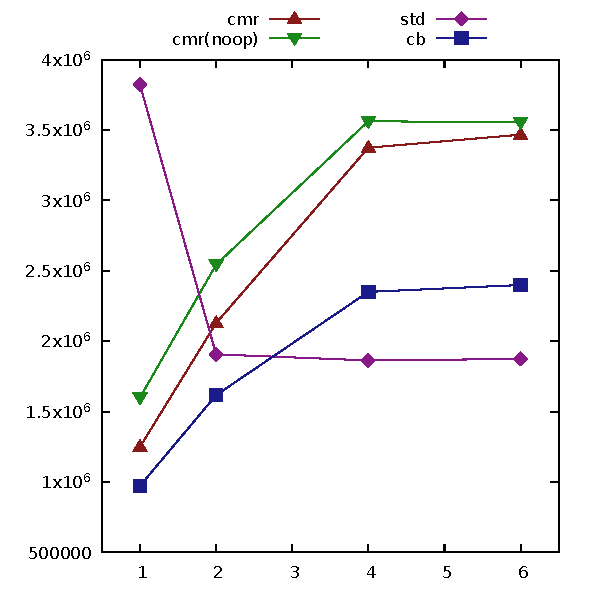
\includegraphics[width=\linewidth]{graphs/lurifax-hm-insert.pdf}
    \caption{Performance of \code{HashMap::insert}}
  \end{subfigure}
  \begin{subfigure}{0.49\linewidth}
    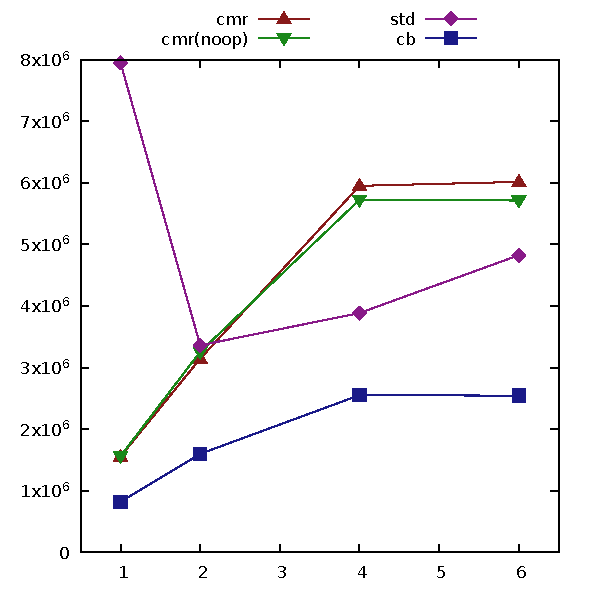
\includegraphics[width=\linewidth]{graphs/lurifax-hm-contains.pdf}
    \caption{Performance of \code{HashMap::contains}}
  \end{subfigure}
\end{figure}

\begin{figure}[ht]
\centering
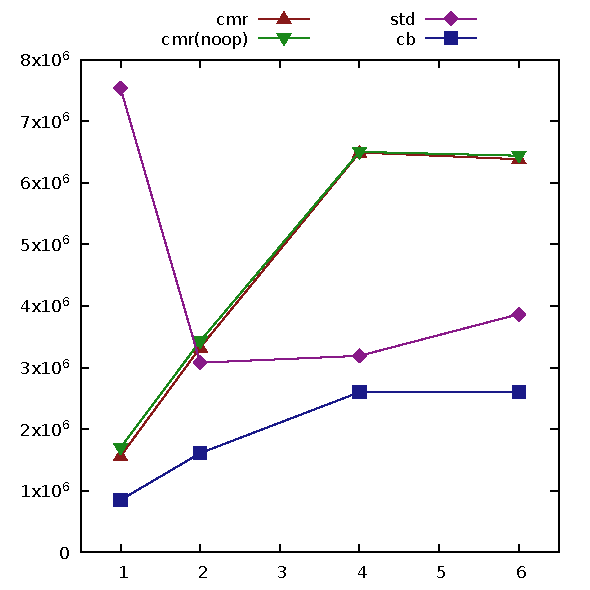
\includegraphics[width=0.49\linewidth]{graphs/lurifax-hm-80-10-10.pdf}
\caption{\code{HashMap} performance with 80\% query, 10\% insert, and 10\% delete.}
\end{figure}


\section{Thirt Party Use}
\lorem{}


\chapter{Conclusion}
\blindtext{}

\section{Is CMR Useful?}
\blindtext{}

\section{Alternatives}
\blindtext{}

\section{Closing Words}
\blindtext{}


\begin{appendices}
\appendix
  \chapter{Extended Results\label{ap:results}}
\end{appendices}

\printglossary[type=\acronymtype,title=Abbreviations]
\printglossary{}

\bibliographystyle{acm}
\addcontentsline{toc}{chapter}{Bibliography}
\bibliography{sources}


\end{document}
